\documentclass[a4paper,12pt,openany,oneside,utf-8]{ctexbook}
\usepackage{amssymb,amsmath}
\usepackage{subcaption}
\usepackage[amsmath,thmmarks]{ntheorem}
\usepackage{fancyhdr}
\usepackage{graphicx}
\usepackage{titletoc}
\usepackage{epsfig,picins,picinpar}
\usepackage{setspace}
\usepackage{geometry}
\geometry{left=3.3cm,right=2.8cm,top=2.5cm,bottom=2.2cm,}
\usepackage{mathtools}
\usepackage[super,square,comma,sort&compress]{natbib}
\usepackage{multirow}
\usepackage{dsfont}
\usepackage{booktabs}
\usepackage{epstopdf, pdfpages}
\usepackage{ccmap}
\bibliographystyle{gbt7714-2005}
\DeclareMathOperator*{\argmax}{arg\,max}
\usepackage{bm}
\usepackage{makecell}
\usepackage{booktabs}
\usepackage{threeparttable}
\usepackage{algorithm}
\usepackage{algorithmicx}
\usepackage{algpseudocode}
\usepackage{titlesec}
\usepackage{indentfirst}
\usepackage{caption}
\floatname{algorithm}{Algorithm}
\renewcommand{\algorithmicrequire}{\textbf{Input:}}
\renewcommand{\algorithmicensure}{\textbf{Output:}}
\usepackage{paralist}


\allowdisplaybreaks[4]
\renewcommand{\baselinestretch}{1.5}
%\renewcommand{\chaptername}{{Chapter\thechapter}}
\renewcommand{\chaptername}{第{\thechapter}章}
\renewcommand\bibname{参考文献}
\renewcommand\contentsname{目录}
%\renewcommand{\sectionname}{{\thechapter}.\arabic{section}}

\renewcommand {\thetable} {\thechapter{}-\arabic{table}} 
\renewcommand {\thefigure} {\thechapter{}-\arabic{figure}}

% 字体大小设置
\newcommand{\chuhao}{\fontsize{48pt}{\baselineskip}\selectfont}
\newcommand{\xiaochuhao}{\fontsize{36pt}{\baselineskip}\selectfont}
\newcommand{\yihao}{\fontsize{28pt}{\baselineskip}\selectfont}
\newcommand{\xiaoyihao}{\fontsize{25pt}{\baselineskip}\selectfont}
\newcommand{\erhao}{\fontsize{21pt}{\baselineskip}\selectfont}
\newcommand{\xiaoerhao}{\fontsize{17pt}{\baselineskip}\selectfont}
\newcommand{\sanhao}{\fontsize{15.75pt}{\baselineskip}\selectfont}
\newcommand{\xiaosanhao}{\fontsize{15pt}{\baselineskip}\selectfont}
\newcommand{\sihao}{\fontsize{13pt}{\baselineskip}\selectfont}
\newcommand{\xiaosihao}{\fontsize{12pt}{\baselineskip}\selectfont}
\newcommand{\wuhao}{\fontsize{10.5pt}{\baselineskip}\selectfont}
\newcommand{\xiaowuhao}{\fontsize{9pt}{\baselineskip}\selectfont}
\newcommand{\liuhao}{\fontsize{7.875pt}{\baselineskip}\selectfont}
\newcommand{\qihao}{\fontsize{5.25pt}{\baselineskip}\selectfont}%\newcommand\kaishu{\CJKfamily{kai}}
%这样在文档中就可以随心所欲地改变字体了, 比如上图中开始部分就是用
% {\yihao 1770年}{\sanhao 法国人狄道} 来实现的

\CTEXsetup[name={第,章}, number=\arabic{chapter}]{chapter} %将目录和正文的"第一章  XXXX"的输出格式改为"第1章 XXXX" see: https://blog.csdn.net/jk123vip/article/details/57163786 and http://tieba.baidu.com/p/3631630597
\titleformat{\chapter}{\centering\sanhao\bfseries}{第\,\thechapter\,章}{1em}{}
\titlespacing*{\chapter} {0pt}{-10.5pt}{12pt}

\titleformat{\section}{\centering\xiaosanhao\bfseries}{\thesection}{1em}{}
\titlespacing*{\section} {0pt}{12pt}{12pt}

\titleformat{\subsection}{\sihao\bfseries}{\thesubsection}{1em}{}
\titlespacing*{\subsection} {0pt}{0pt}{5.25pt}

\DeclareCaptionFont{fivehao}{\fontsize{10.5pt}{11pt}\selectfont #1} 
\pagestyle{fancy}%
%\renewcommand{\headrulewidth}{0pt}       %把页眉线的宽度设为零, 即去掉页眉线
\renewcommand{\footrulewidth}{0pt}
\addtolength{\headheight}{0\baselineskip}
\addtolength{\headwidth}{0\marginparsep}
\addtolength{\headwidth}{0\marginparwidth}
\setlength{\headsep}{5mm}
\fancyhf{}


\begin{document}
\theoremstyle{plain} \theoremseparator{}
\theoremindent0cm\theoremnumbering{arabic} \theoremsymbol{}% 以上是latex 的默认设置

%\vskip 26pt
%\renewcommand\refname{\Large\bf References}

%%%%%%%%%%%%%%%%%%%%%%%%%%%%%%%%%%%%

\fancypagestyle{plain}{%
\fancyhead{} 
% clear all header fields
%\fancyhead[CE,CO]{\xiaowuhao{浙江工商大学硕士学位论文}}} %上传到系统里面的论文电子最终版本不要出现页眉(就是每一页的最顶端不要再写浙江工商大学了)
\fancyhead[CE,CO]{\xiaowuhao{}}} 
%上传到系统里面的论文电子最终版本不要出现页眉(就是每一页的最顶端不要再写浙江工商大学了)
\begin{titlepage}
\fancypagestyle{plain}{\pagestyle{fancy}}
%\fancyhead[C]{\xiaowuhao 浙江工商大学硕士学位论文} % 上传到系统里面的论文电子最终版本不要出现页眉(就是每一页的最顶端不要再写浙江工商大学了)
\fancyhead[C]{\xiaowuhao} % 上传到系统里面的论文电子最终版本不要出现页眉(就是每一页的最顶端不要再写浙江工商大学了)
%%%%%%%%%%%%%%%%%%%%%%%%%%%%%%%%%%%%%%%%%%%%%%%%%%%%%%%%%%%%%%%%%%%%%%%%%%%% 完整
\vskip 4mm
\xiaowuhao 密级:公开 \hspace{9cm}中图分类号:O212.1

\vskip 6mm

\begin{figure}[htbp]
\centering

\includegraphics[width=140mm,height=22mm]{figures/zjgsu.jpg}
\end{figure}

\vskip 10mm

\begin{spacing}{1.0}
\begin{center}
\chuhao\textbf{硕士学位论文}
\end{center}

\vskip 20mm
\begin{center}
\hspace{0.01mm}\sanhao\textbf{论文题目:\underline{基于扩散模型的三维药物分子设计框架}}
\end{center}
\end{spacing}
\vspace{24mm}

\begin{center}
\textbf{\kaishu\sanhao 作者姓名:\underline{\quad \quad \quad \quad  徐璨 \quad \quad \quad \quad}}
\end{center}


\begin{center}
\textbf{\kaishu\sanhao 学科专业:\underline{\quad \quad \quad \ \ 统计学 \ \ \quad \quad \quad}}
\end{center}


\begin{center}
\textbf{\kaishu\sanhao 研究方向:\underline{\quad \quad \ \ \ 数理统计 \ \ \ \ \quad \quad}}
\end{center}

\begin{center}
\textbf{\kaishu\sanhao 指导教师:\underline{\quad \quad \quad \ \  王伟刚 \ \ \quad \quad \quad  }}
\end{center}

\

\

\


\begin{center}
\kaishu\sanhao 提交日期:2024 年 1 月
\end{center}
\end{titlepage}

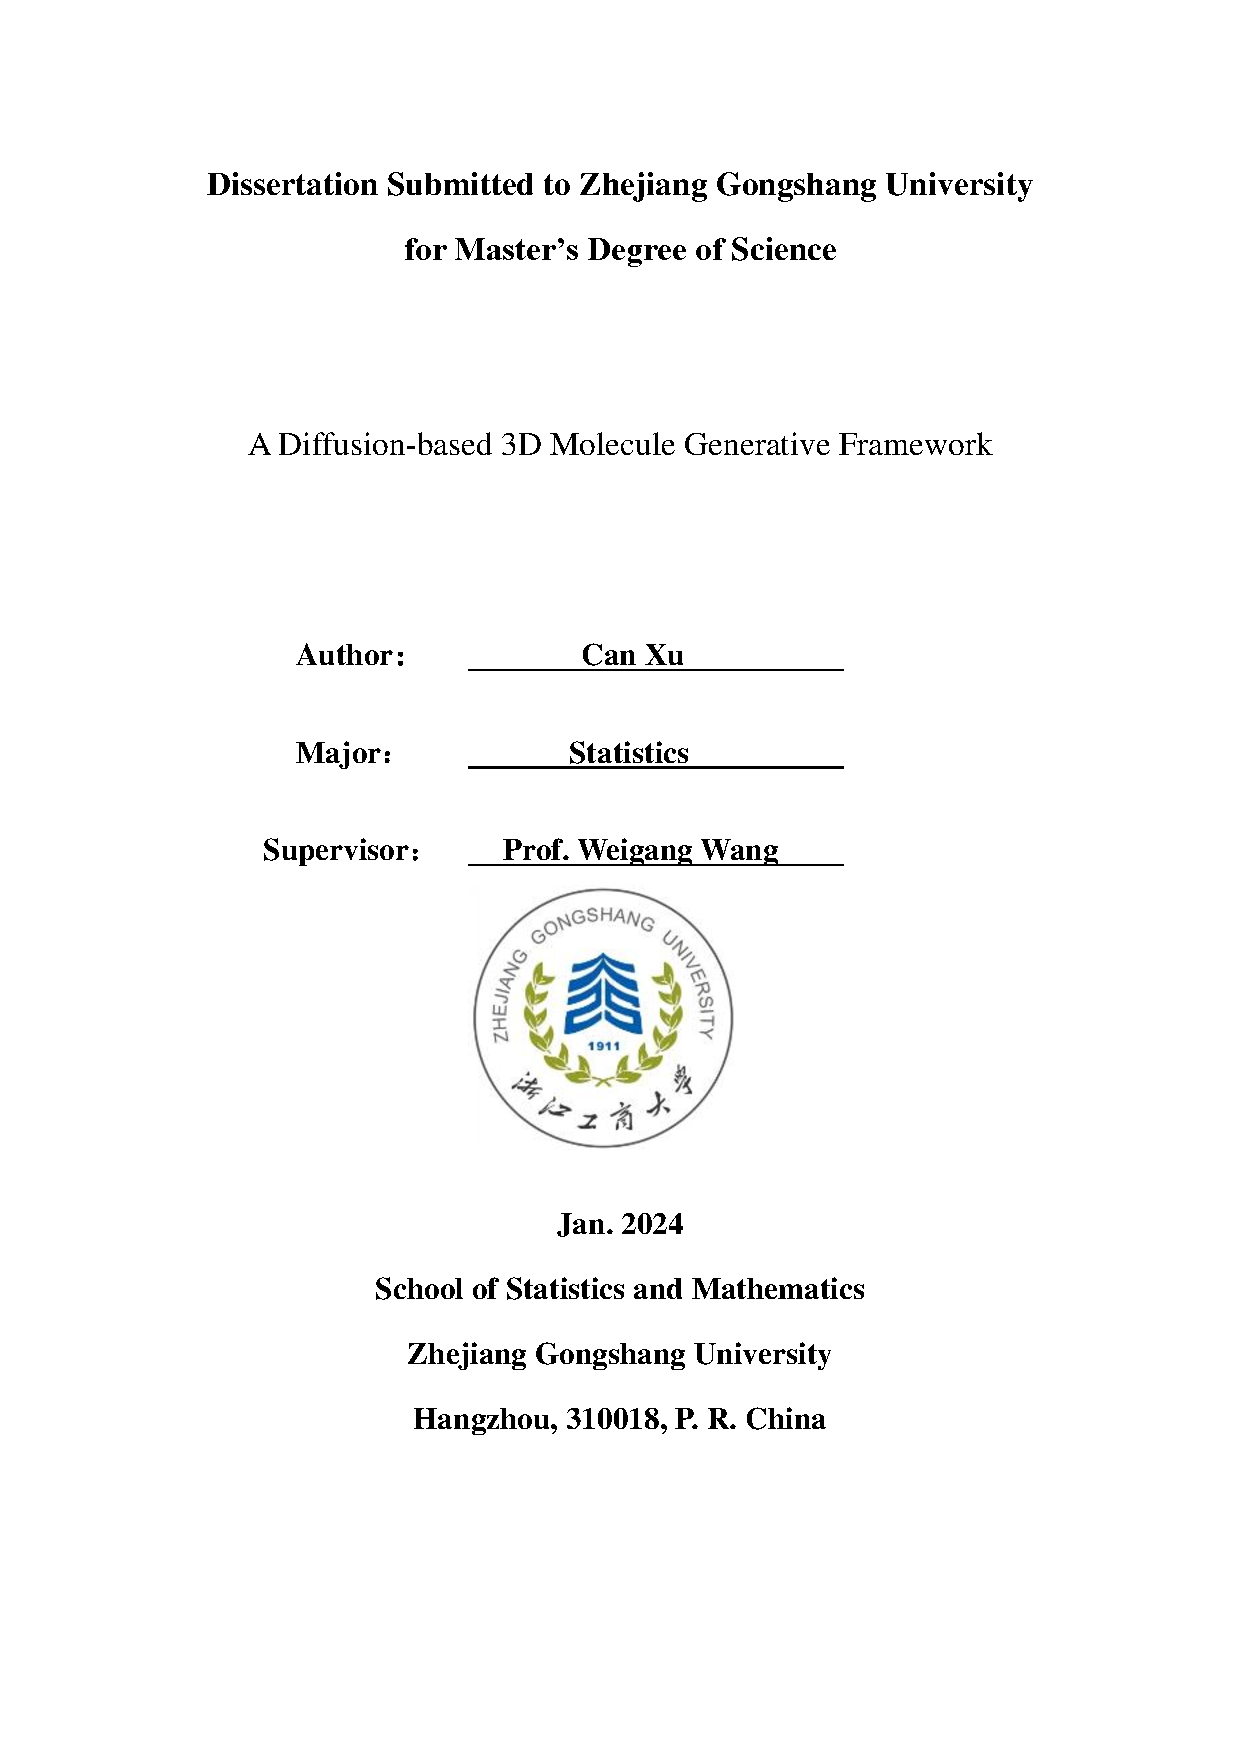
\includepdf{figures/covers/cover_en.pdf}

% 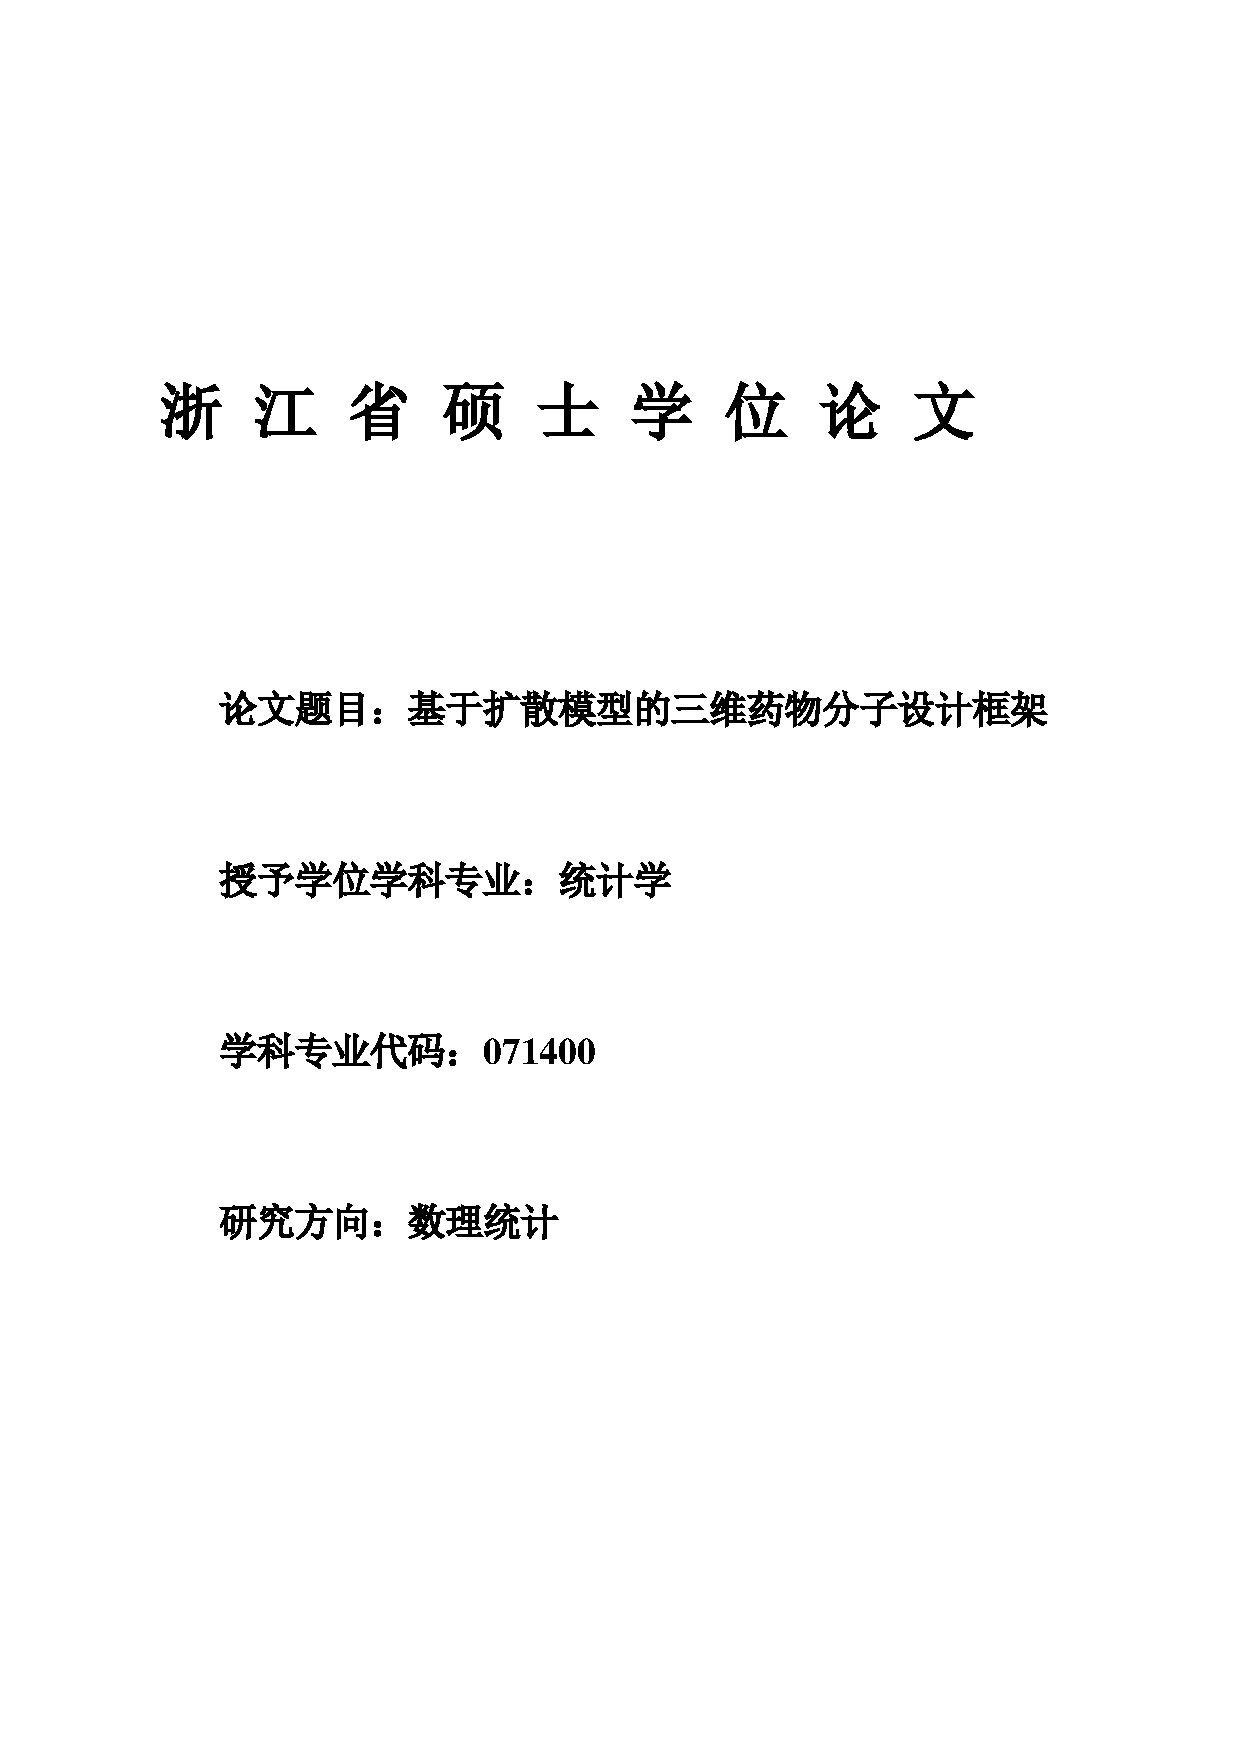
\includepdf{figures/covers/cover_anonymous.pdf}

\frontmatter
\pagenumbering{Roman}
\cfoot{\thepage}
\newpage
% \begin{center}
% \heiti\sanhao{\textbf{基于扩散模型的三维药物分子设计框架}}
% \end{center}
% \vskip 10 mm
\begin{center}
\heiti\sanhao{\textbf{摘 \quad 要}}
\end{center}
\vskip 7 mm
\begin{spacing}{1.5}
{\sihao 去噪扩散模型在多个研究领域显示出巨大潜力。现有的基于扩散生成模型在全新的三维分子生成任务中面临两个主要挑战。由于分子中的大部分重原子能够通过单键与多个原子相连,使用成对距离来建模分子几何结构是不足够的。因此,第一个挑战是提出一个有效的神经网络作为去噪核,能够捕捉复杂的原子间关系并学习高质量的特征。此外,由于图的离散性质,当前主流的基于扩散分子生成模型严重依赖预设的规则,并以间接的方式生成边。故第二个挑战是将分子生成的过程与扩散的学习过程相结合,有效地准确预测键的存在。本文认为扩散过程中分子构象的迭代更新方式与分子动力学一致,故提出一种名为几何辅助的分子扩散(Geometric-facilitated Molecular Diffusion / GFMDiff)的新型分子生成框架。针对第一个挑战,我们引入了一种双轨Transformer网络(Dual-track Transformer Network / DTN),以全面挖掘全局空间关系并学习高质量的表示,从而提高对特征和几何结构的准确预测能力。至于第二个挑战,我们设计了几何辅助损失(Geometric-facilitated Loss / GFLoss),该损失在训练期间干预键的形成,而不是直接将边嵌入隐变量空间。本文在多个基准数据集上开展了全面实验表明GFMDiff性能达到该领域时下最优的水平。}
\end{spacing}
% \begin{spacing}{1.8}
% {\sihao 在智能计算的计算医药相关研究中,深度学习模型在药物发现、药物属性预测等应用中已经展现出良好的性能和极大的潜力。人工智能技术应用能够为药物研发的多个阶段降本增效。过去的2022年,AI制药赛道相关融资总金额达百亿美元。国内互联网巨头如百度百图生科、华为EIHealth、腾讯云深智药,及初创企业晶泰科技,剂泰医药,星药科技等,相关成果已经展现出深度学习在该领域的强大性能和广阔前景。}
% \end{spacing}
% \begin{spacing}{1.8}
% {\sihao 近来大火的生成模型被广泛应用于智能计算领域,人工智能算法有望根据人类的要求生成理想的结果,帮助提升药物发现与设计的效率与质量。在计算化学的相关研究中,深度学习模型的成功落地能够推动制药企业减少湿实验成本,助力靶点确认、药物发现、分子生成、化学反应设计、化合物筛选、临床试验、风险评估等多阶段。}
% \end{spacing} 
% \begin{spacing}{1.8}
% {\sihao 本文聚焦于深度学习算法在三维药物分子发现这一主题,意在利用时下最优的生成模型算法,创新性设计出更符合三位药物理化性质的算法,提升全新药物分子设计的性能与效率。}
% \end{spacing}
\vskip 16 mm
\noindent {\sihao 关键词: 扩散模型;分子生成;分子学习;图神经网络;几何神经网络}


%%%%%%%%%%%%%%%%%%%%%%%%%%%%%%%%%%%%%%%%%%%%%%%%%%%%%%%%%%%%%%%%%%%%%%%%%%%%%%%%%%%%%%%%%%%%%%%%%%%%%%%%
                                                                                                       %
\newpage                                                                                               %
% \begin{spacing}{1.1}
% \begin{center}
% \heiti\sanhao{\textbf{A DIFFUSION-BASED 3D MOLECULE GENERATIVE FRAMEWORK}}
% \end{center}
% \end{spacing}
% \vskip 14mm
% \vskip 7mm
\begin{center}
\heiti\xiaosanhao{\textbf{Abstract}}
\end{center}
\vskip 7mm

\begin{spacing}{1.5}
{\sihao Denoising diffusion models have shown great potential in multiple research areas. Existing diffusion-based generative methods on {\itshape de novo} 3D molecule generation face two major challenge. Since majority heavy atoms in molecules allow connections to multiple atoms through single bonds, modeling molecule geometries using pair-wise distance is insufficient. Therefore, the first one involves proposing an effective neural network as the denoising kernel that is capable to capture complex interatomic relationships and learn high-quality features. Due to the discrete nature of graphs, mainstream diffusion-based methods for molecules heavily rely on predefined rules and generate edges in a indirect manner. The second one involves accommodating molecule generation to the learning process of diffusion and accurately predicting the existence of bonds effectively. In our research, we view the iterative way of updating molecule conformations in diffusion process is consistent with molecular dynamics and introduce a novel molecule generation method named Geometric-Facilitated Molecular Diffusion (GFMDiff). For the first challenge, we introduce a Dual-track Transformer Network (DTN) to fully excevate global spatial relationships and learn high quality representations which contribute to accurate predictions of features and geometries. As for the second challenge, we design Geometric-facilitated Loss (GFLoss) which intervenes the formation of bonds during the training period, instead of directly embedding edges into the latent space. Comprehensive experiments on current benchmarks demonstrate the superiority of GFMDiff.}
\end{spacing}

\vskip 14 mm
\noindent{KEYWORDS: Diffusion models; Molecule generation; Molecular learning; Graph neural networks; Geometry neural Networks}

\newpage
\begin{spacing}{1.5}
\tableofcontents
\titlecontents{chapter}[0pt]{\addvspace{2pt}\filright}
{\contentspush{\thecontentslabel\ }}
{}{\titlerule*[8pt]{.}\contentspage}
\end{spacing}

\mainmatter
\fancyfoot[EC,OC]{\hspace*{1 em}\thepage{}\hspace*{1 em}}
\normalsize
\fancypagestyle{plain}{\pagestyle{fancy}}
%\chapter[引言]{引言}\fancyhead[C]{\xiaowuhao 浙江工商大学硕士学位论文} %上传到系统里面的论文电子最终版本不要出现页眉(就是每一页的最顶端不要再写浙江工商大学了)
\chapter[引言]{引言}\fancyhead[C]{\xiaowuhao} %上传到系统里面的论文电子最终版本不要出现页眉(就是每一页的最顶端不要再写浙江工商大学了)
\section{选题背景与研究意义}
\subsection{选题背景}
除图像、视频,音频与自然语言处理等领域,AI技术的快速发展也带动相关交叉学科的发展。AI4Science近年在计算生物、计算化学、材料设计、计算天文,计算育种等都有广泛应用,相关AI技术的应用能够大幅加速相关科学研究进展。在计算制药领域,近年来相关AI技术在药物性质预测,生成,开发,实验等领域的运用不仅加速相关研究的进展,也能够降低相关研究的研发成本。

基于AI的生成模型近十年来也被广泛研究,他们包括变分自编码器(Variational autoencoders / VAEs)\cite{vae_kingma_13},生成对抗模型(Generative adversarial networks / GANs)\cite{gan_goodfellow_14},流形模型(Normalizing flows / NFs)\cite{nice_dinh_15,density_dinh_17},自回归(Autoregressive models / ARs)\cite{ar_oord_16}与扩散模型(Diffusion)\cite{deepunsupervised_dickstein_15,generative_song_19}等。相关方法在图像,文字等方面也有了许多成功应用。

深度学习在分子化学领域近年来也有着成功的应用。以分子学习为例,化学分子常以简化分子线性输入规范字符串(Simplified molecular-input line-entry system / SMILES)\cite{smiles_weinberger_88}存储,每一个分子式对应一个SMILES字符串。随着早期深度学习方法,如卷积神经网络(Convolutional neural networks / CNNs)\cite{cnnsmiles_hirohara_18}和循环神经网络(Recurrent neural networks / RNNs)\cite{rnnsmiles_bjerrum_17,practicalmodel_liu_19,deeppurpose_huang_20}的发展,一些研究试图运用这些深度学习算法,对以字符串形式存在的分子式进行学习,以获得预测特定原子或是分子整体的性质的能力。随着图神经网络(Graph neural networks / GNNs)\cite{semisupervised_kipf_17,inductive_hamilton_17,howpowerful_xu_18}的出现,其对非结构化数据的建模能力和对节点间拓扑关系学习的能力被证明十分优异。分子作为自然界中天然存在的图结构,原子和键对应着图中的节点和边,这为分子学习提供了新的思路与方法。从最早的图卷积神经网络开始,相关研究者致力于提出新的图学习算法,以提升对分子图学习的性能。随着相关化学模拟技术的发展,让三维分子建模成为可能。这也在拓扑结构信息以外,提供了更丰富的几何构型信息,这也驱动着相关研究拓展至几何图神经网络上。分子三维构象允许研究者对分子进行更准确的研究,同时也推动更多复杂任务的出现,包括分子生成,Ligand生成,Protacs生成,药物亲和力预测,蛋白质预测等等。

\subsection{研究意义}
人工智能在智能计算相关研究中开始扮演越来越重要的角色,相关模型在药物发现、药物属性预测等应用中已经展现出良好的性能和极大的潜力。由于深度学习技术应用具备为药物研发的多阶段降本增效的潜力,在2022年,AI制药赛道相关企业融资总金额达百亿美元。在这一赛道竞逐的有国内互联网巨头如百度百图生科、华为EIHealth、腾讯云深智药,及初创企业晶泰科技,剂泰医药,星药科技等。相关成果已经展现出深度学习在该领域的强大性能和广阔前景。

\section{文献综述}
\subsection{基于深度学习的分子学习}
分子最早被表示为简化分子线性输入规范字符串(SMILES)\cite{smiles_weinberger_88},随着早期深度学习模型卷积神经网络(CNN)和循环神经网络(RNN)的发展,相关模型利用CNNs和RNNs对分子性质做出学习。Hirohara等\cite{cnnsmiles_hirohara_18}的研究提出使用CNN对分子级别的特征和分子基团性质进行有效学习。由于RNNs在早期自然语言护理任务上有良好表现,Bjerrum\cite{rnnsmiles_bjerrum_17}提出LSTM-QSAR模型用于学习分子性质。

伴随图神经网络(GNNs)的发展,由于分子的形式天然的属于图结构,一些研究开始使用GNNs进行分子学习。CGCNN\cite{cgcnn_xie_18}将图卷积神经网络引入到分子性质学习,用以模拟并替代复杂的DFT计算。Xiong等\cite{attentivefp_xiong_20}提出Attentive FP,一个结合注意力机制的图神经网络实现分子性质的有效学习与预测。GraSeq\cite{graseq_guo_20}提出在运用图神经网络学习拓扑结构同时,利用双向LSTM模型对SMILES分子式进行学习,通过两个通道联合预测分子性质。伴随相关技术的发展,研究者可以不再拘泥于原子拓扑结构,进而实现对分子三维结构的建模与学习。鉴于某一分子对应大量的同分异构体,而不同构象对应属性不尽相同,因此对三维构象的有效学习是十分必要的。EGNN\cite{egnn_satorras_21}在流行的图网络基础上,保留最基本的几何信息,即原子间距离,其简单的设计也成为了一些。在分子预训练框架GEM\cite{gem_fang_22}中,研究者提出GeoGNN图网络,将键长视作原子节点图的边特征,又对原子键构图,并将键角作为原子键图的边特征,通过在两个网络上的信息传递实现分子局部空间几何性质学习。Sch\"{u}tt等\cite{schnet_schutt_17}在继承GNNs的信息传递范式的同时,将原子间距离用径向基函数(Radial basis funciton / RBF)建模后融入边特征,使算法对三维几何信息的有效学习的同时保证了等变性要求。SphereNet\cite{spherenet_liu_22}提出了基于球坐标系的信息传递范式SMP。通过一系列参考原子或键的规则,SMP在保证对原子对距离,键角和键扭转角这三个空间几何信息完整提取的同时,避免计算复杂度的爆炸式增长。ComENet\cite{comenet_wang_22}在ShpereNet的基础上,简化了空间几何信息的提取范式,在保证利用完整空间信息的前提下,以损失部分精度为代价,大幅度提升计算速度。

伴随着Transformer\cite{transformer_vaswani_17}相关研究在图像与文本领域的兴起,相关研究\cite{smilestrans_honda_19,smilesbert_wang_19,chemberta_chithrananda_20}也利用Transformer对SMILES分子式进行学习。随着GTN\cite{gtn_yun_19}将Transformer引入图学习,越来越多的研究也将多头注意力机制用于分子图学习领域。大规模分子图预训练框架GROVER\cite{grover_rong_20}中,分子学习内核运用了GTransformer,同时学习分子中的原子与键的节点嵌入(embedding)或边嵌入。在分子预训练框架MPG\cite{mpg_li_21}中提出的图学习内核MolGNet放弃了对边嵌入的学习,仅利用多头注意力学习节点嵌入,结果证明了该图学习算法的有效性。

\subsection{基于深度生成模型的分子设计}
自深度学习研究兴起以来,深度生成模型一直是研究者重点研究的对象。作画、翻译、对话,渲染等应用能够直接服务于广大用户。主流的深度生成模型有变分自编码器(Variational autoencoders / VAEs)\cite{vae_kingma_13},生成对抗模型(Generative adversarial networks / GANs)\cite{gan_goodfellow_14},流形模型(Normalizing flows / NFs)\cite{nice_dinh_15,density_dinh_17},自回归(Autoregressive models / ARs)\cite{ar_oord_16}与扩散模型(Diffusion)\cite{deepunsupervised_dickstein_15,generative_song_19}等。

与图学习的演进过程相似,基于深度生成模型的分子设计也经历了从二维图结构到三维几何构象的演进。主流分子设计任务具体又可以被细分为:分子生成,分子优化,构象生成,蛋白质配体生成,蛋白质生成,蛋白降解靶向嵌合体生成。

分子生成的任务就是根据给定分子数据,使模型具备凭空生成全新且有效的药物分子图或三维结构。考虑到复杂药物分子主要由官能团等子结构组成,JT-VAE\cite{jtvae_jin_18}基于VAE生成树结构骨架,而后利用树结构骨架逐步生成分子图结构。GraphVAE\cite{graphvae_simonovsky_18}是早期的基于VAE的图生成研究,为避免离散化结构的线性表示的相关障碍,使其中解码器直接输出预设的最大概率的全连接图。基于NF模型,MoFlow\cite{moflow_zang_20}将隐式表征逐步映射到条件流过程中,模型首先生成连接原子的键,随后通过图条件流生成原子,并最终组成有效的分子图。

现有的基于扩散的分子生成模型有且只有EDM\cite{edm_hoogeboom_22}和MDM\cite{mdm_huang_22}。
 
\section{创新点}
本文聚焦于扩散模型在分子生成领域的前沿研究,意在提出一个能够设计出有效、稳定分子的生成模型框架。本文利用扩散模型作为生成框架的骨架,在扩散模型的去噪内核设计上,本文提出了一个全新的图学习算法。该算法能够对几何信息,拓扑信息和原子化学性质进行分别建模,在保证模型等变形的条件下,实现对多种信息的有效学习与利用。

\section{基本框架}

\chapter[分子图学习与基于扩散模型的图生成]{分子图学习与基于扩散模型的图生成}
\label{chap:diffusion-based_molgen}

\section{分子图学习}
在图学习中通常有两类监督任务:节点分类/回归和图分类/回归。对于图学习,一个分子可以被抽象为一个图 $\mathcal{G} = (\mathcal{V}, \mathcal{E})$,其中 $|\mathcal{V}| = n$表示节点(原子)的集合,$|\mathcal{E}| = m$ 表示分子中的边(化学键)的集合。我们用$e_i$表示节点 $i$的特征,用$e_{ij}$表示边$(i, j)$的特征。

在节点分类或回归任务中,每个节点$i$都有一个标签或目标$y_i$。任务目标是通过学习,预测未见节点的标签。这个任务可被应用于许多应用,比如识别分子中的功能团或预测各个原子的性质。

此外,在图分类或回归任务中,给定一组图$\{ \mathcal{G}_1, \mathcal{G}_2, ..., \mathcal{G}_N \}$和对应的标签或目标 $\{ y_1, ..., y_N \}$。此时任务目标是根据图的结构和节点边的特征,预测给定图的标签或目标。这个任务被广泛应用于化合物分类或基于结构预测分子性质等。

在这两类任务中,目标是利用监督学习技术训练模型,有效地捕捉图的结构与相关标签/目标之间的关系。现有的图学习方法主要有基于图神经网络的模型和基于Transformer架构的模型。

图神经网络(Graph Neural Networks,简称GNNs),近来在知识图谱、社交网络和药物发现等各个领域引起了广泛的关注。GNNs的核心操作在于将图中节点或边之间的特征进行传递(也称为邻居聚合)。消息传递操作通过聚合节点$i$的邻居节点和边的隐式特征来迭代更新节点$i$自身的隐式特征$e_i$。一般来说,消息传递过程包含多轮迭代,每轮迭代可以被视为对更远距离邻居的消息聚合。假设有$L$轮迭代,第$l$轮迭代会将目标节点的l跳邻居特征注入目标节点的隐式特征。第$l$轮迭代中,消息的传递与聚合可被表示为:
\begin{eqnarray}
    &m_j^{(l)} = {\rm MSG}^{(l)}(e_j^{(l-1)}), \ j \in \mathcal{N}_i, & \\
    &e_i^{(l)} = {\rm AGG}^{(l)}(\{ m_j^{(l)}, \ j \in \mathcal{N}_i \}, \ m_i^{(l)} ), &
\end{eqnarray}
其中$m_j^{(l)}$为聚合后的消息,MSG为消息聚合函数,主流的选择包括多层感知机(MLP),可学习权重。$e_i^{(l)}$为聚合后的目标节点特征,AGG为聚合函数,主流的方式有平均值池化、最大池化和图注意力机制等。对每一次消息传递,MSG和AGG函数都可能存在可训练的参数,这些参数在每轮迭代中一般是共享的。经过$L$次消息传递与聚合后,最后一次迭代后的隐式特征被视为模型预测的节点嵌入,即$e_i^{(L)}$。最后,根据具体任务需要,运用相应的READOUT函数即可得到节点信息或是全图级别的信息。

近年来,伴随Transformer模型的出现,一些研究也开始将该架构引入图学习中。多头注意机制是Transformer的核心模块,它将多个注意力层堆叠在一起,实现并行运算。一个注意力层的核心要素一般为一组查询、键、值组成,记为$(\mathbf{Q}, \mathbf{K}, \mathbf{V})$。通过查询和键的点积,经过softmax函数归一化后即可获得注意力概率,具体可表示为:
\begin{eqnarray}
    {\rm Attention}(\mathbf{Q}, \mathbf{K}, \mathbf{V}) = {\rm softmax}(\frac{\mathbf{Q} \cdot \mathbf{K}^T}{\sqrt{d}}) \cdot \mathbf{V},
\end{eqnarray}
其中$d$为注意力头数。

\section{等变性要求}

\section{基于扩散模型的图生成}
扩散模型在生成模型中引起了相当大的关注。通过学习逆过程的去噪核,这些模型能够揭示噪声样本的潜在分布。在给定一段数据的情况下,正向过程被视为马尔可夫链,通过学习可学习参数控制噪声强度,逐渐向数据添加高斯噪声$T$次。在生成过程中,模型将噪声还原回真实数据的原始分布。

\subsection{扩散过程}
设$G_t (t=0, 1, ..., T)$表示分子几何信息的分布,$\beta_t \in (0, 1), t=0, 1, ..., T$表示马尔可夫链的噪声方差序列。因此我们可以得到几何信息在$t$或$T$时刻在后验分布:
\begin{eqnarray}
&q(G_{1:T} | G_0) = \prod^T_{t=1} q(G_t | G_{t-1}), & \\
&q(G_t | G_{t-1}) = \mathcal{N}(G_t; \sqrt{1-\beta_t}G_{t-1}, \beta_t I).&
\end{eqnarray}

随着时间步$t$的增加,扩散过程逐步将更多的噪声添加到原始数据分布,具体表现为噪声方差$\beta_t$从0平滑地过渡到1。设$\bar{\alpha}_t = \prod^t_{s=1} \alpha_s = \prod^t_{s=1}(1-\beta_s)$,则任意$t$时刻样本数据的分布可以表示为:
\begin{equation}
    q(G_t|G_0) = \mathcal{N}(G_t; \sqrt{\bar{\alpha}_t} G_0, (1 - \bar{\alpha}_t) I).
\end{equation} 

\subsubsection{去噪过程}
在去噪过程中,模型通过学习接近真实的逆过程$q(G_{t-1} | G_t)$的马尔可夫核函数$p_\theta(G_{0:T-1}| G_{T}) = \prod^T_{t=1} p_\theta(G_{t-1} | G_t)$来重新构建原始的几何信息。每个时间步中学习到的去噪分布为: 
\begin{equation}
  p_\theta(G_{t-1} | G_t) = \mathcal{N}(G_{t-1}; \mu_\theta(G_t, t), \sigma_t^2 I),
\end{equation}
其中$\mu_\theta(G_t, t)$是可训练的神经网络,被用于近似估计均值,$\sigma^2_t = \frac{(\beta_t - \beta_{t-1})\beta_{t-1}}{(1 - \beta_{t-1}) \beta_t}$是预定义的方差。在采样过程开始时,$p_\theta(G_T)$采样自标准高斯分布中,然后通过迭代的去噪过程逐步优化参数化的神经网络,并最终到达0时刻得到几何信息的采样结果。

理论上,神经网络的目标函数采用数据的对数似然函数的变分下界形式:
\begin{eqnarray}
    &{\rm log}p(G) \geq \mathcal{L}_{base} + \sum_{t=0}^T \mathcal{L}_t,& \\
    &\mathcal{L}_{base} = -KL(q(G_T|G_0)|p(G_T)),& \\
    &\mathcal{L}_t = KL(q(G_{t-1}|G_t)|p(G_{t-1}|G_t)). &
\end{eqnarray}
然而,研究发现,神经网路预测的高斯噪声$\epsilon$能够更容易的用于训练。因此,在实际优化神经网络时,神经网路的目标函数$\mathcal{L}_t$ \cite{vaediff_kingma_21}的形式为:
\begin{equation}
    \mathcal{L}_t = E_{\epsilon_t \sim \mathcal{N}(0, I)}[\frac{1}{2}(1- \frac{{\rm SNR}(t-1)}{{\rm SNR}(t)})||\epsilon_t - \hat{\epsilon}_t||^2].
\end{equation}



\chapter[几何促进的3D分子图生成]{几何促进的3D分子图生成}
\label{chap:gfmdiff}

在本节中,本文将着重介绍3D分子生成的模型框架,具体包括本文提出的E(n)等变去噪内核,几何信息促进的损失函数,扩散及去噪过程和优化目标。本文提出的3D分子生成整体框架由图~\ref{fig:gfmdiff}所示。

\begin{figure}[h]
    \centering
    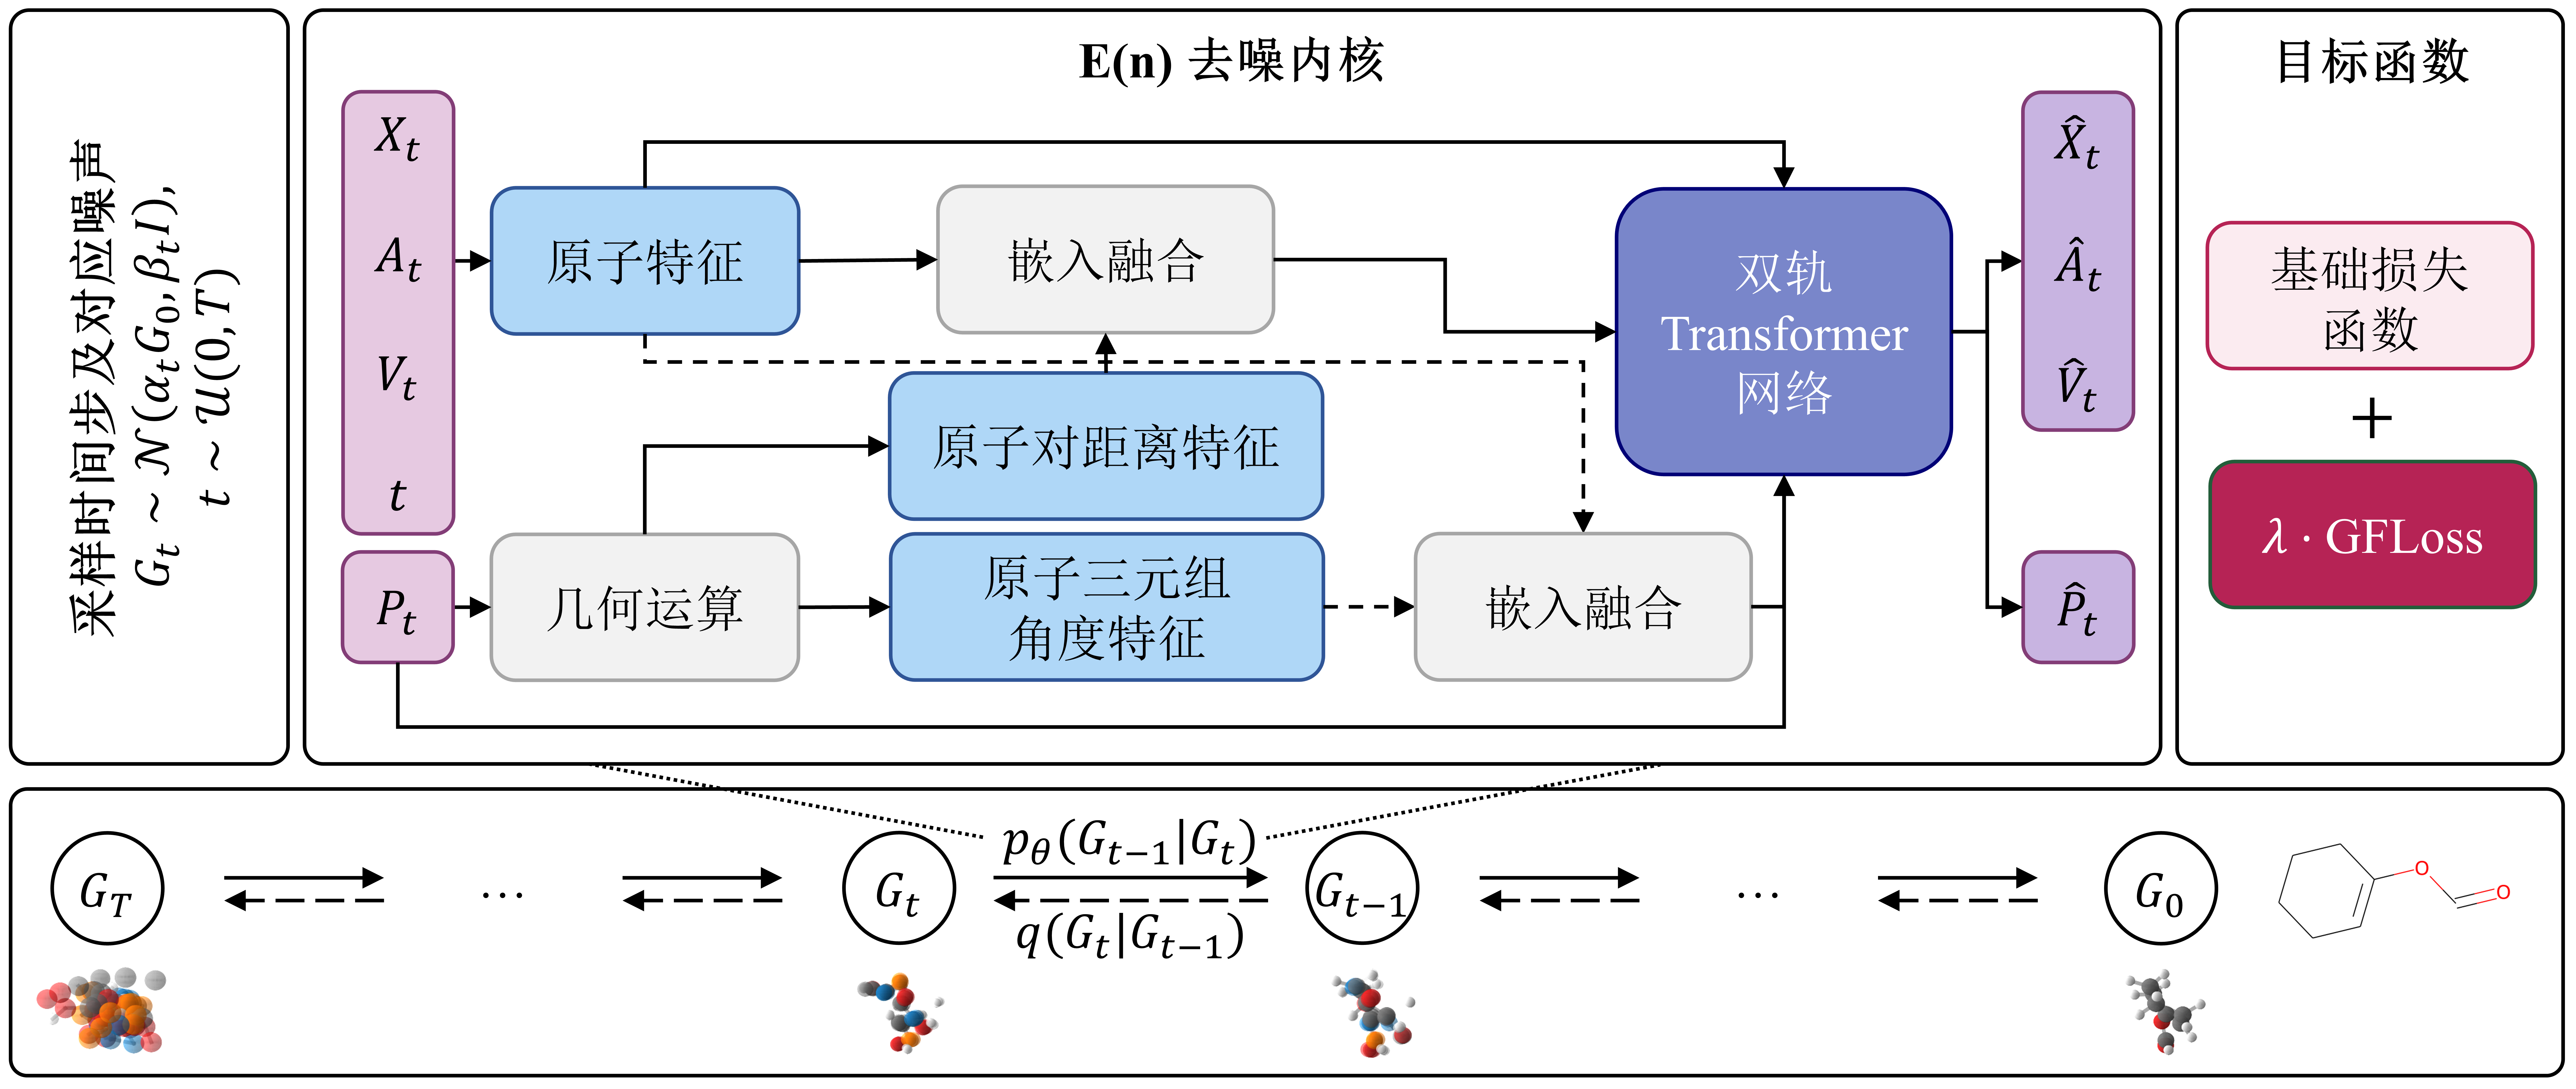
\includegraphics[width=\linewidth]{figures/overview_gfmdiff.png}
    \caption{GFMDiff模型框架示意图}
    \label{fig:gfmdiff}
  \end{figure}

在每次训练时,我们随机选取时间步$t$,并对该时刻的噪声分布进行采样,作为E(n)等变的去噪内核的输入。该输入可以总体分为原子特征和其空间坐标。通过本文设计的双轨Transformer网络(Dual-track Transformer Network,简称DTN),我们即可得到网络预测样本在$t-1$时刻的分布。

\section{双轨Transformer网路(DTN)}

在这个小节中,我们将详细介绍作为GFMDiff的E(n)等变去噪内核的双轨Transformer网络(Dual-track Transformer Network,简称DTN)。DTN被设计用于有效捕捉原子之间的关系和原子特征。由于三维分子几何具有旋转、平移、反射和排列等不变性质,使得去噪核满足这些性质是很重要的。所提出的DTN不仅是E(n)等变的,还能充分利用空间信息。

\begin{figure}[h]
  \centering
  
\includegraphics[width=\linewidth]{figures/structure_dtn.png}
  \caption{双规Transformer网络(Dual-track Transformer Network,简称DTN)的示意图}
  \label{fig:dtn}
\end{figure}

% 传统的图神经网络用于学习图结构数据的拓扑信息,仅仅是置换等变的。尽管已经有许多努力致力于赋予GNN上述性质,我们提供了另一种解决这个问题的视角。

在我们提出的方法中,我们将具有总原子数$N$的输入分子视为$G = (P, X, A, V)$,其中$P = (p_1, p_2, ..., p_N) \in \mathbb{R}^{N \times 3}$表示原子坐标,$X = (x_1, x_2, ..., x_N) \in \mathbb{R}^{N \times nf}$表示原子编号的独热编码,$A = (a_1, a_2, ..., a_N) \in \mathbb{R}^{N}$表示原子编号,$V = (v_1, v_2, ..., v_N) \in \mathbb{R}^{N}$表示原子的价数。为了确保等变性,DTN利用成对距离和三元角度来捕捉几何信息。原子$i$和$j$之间的欧几里得距离,反映了原子间相互作用的强度,可以通过以下公式获得:
\begin{equation}
    d_{ij} = ||p_i - p_j||_2.
\end{equation}
在采样阶段,由于原子之间的复杂关系,仅使用成对距离是不足以提取空间信息的。因此,我们进一步使用以下公式计算三元角度:
\begin{equation}
    \varphi_{ijk} = \arccos (\frac{(p_i - p_j) \times (p_i - p_k)}{||p_i - p_j||_2 \times ||p_i - p_k||_2}). 
\end{equation}
上述几何计算使我们能够获得等变的成对和三个嵌入:
\begin{eqnarray}
    &e_{ij} = {\rm Linear}({\rm RBF}(d_{ij}), e_i, e_j),& \\
    &e_{ijk} = {\rm Linear}({\rm RBF}(\varphi_{ijk}), e_i, e_j, e_k),&
\end{eqnarray}
其中$e_i = {\rm Embedding}(x_i, a_i, v_i)$是原子$i$的节点嵌入,结合了原子编号和价数。这些特征随后被输入到具有$L$层的DTN中。

DTN的每一层由以下组件组成:原子对轨道、对-三元轨道和连接模块。原子对轨道模拟了原子之间的相互作用力对目标原子的影响,而对-三元轨道模型则模拟了潜在键角对边的影响。连接模块作为两个轨道之间的桥梁,将原子特征注入到成对特征中,以促进更好的表示学习。

原子对轨道涉及预测其他原子和原子之间相互作用力对目标原子的影响。该轨道以原子嵌入$e_i$和对嵌入$e_{ij}$作为输入:
\begin{eqnarray}
    &e_i = {\rm LayerNorm}(e_i), \ e_{ij} = {\rm LayerNorm}(e_{ij}),& \\
    &\mathbf{Q}_i = {\rm Linear}(e_i), \ \mathbf{K}_i = {\rm Linear}(e_i) + {\rm Linear}(e_{ij}),& \\
    &a_i = {\rm Dropout}({\rm softmax} \frac{\mathbf{Q}_i \mathbf{K}_i^T}{\sqrt{d_h}}), & \\
    &\mathbf{V}_i = {\rm Linear}(e_{ij}) + {\rm Linear}(e_{i}) + {\rm Linear}(e_{j}),& \\
    &\hat{e}_i = {\rm Linear}(a_i \mathbf{V}_i^T),&
\end{eqnarray}
其中$d_h$是头的数量。原子嵌入首先通过添加原子对轨道的预测来更新,然后传递给前馈网络。在每一层中,原子吸收其他原子和相应的原子对的聚合表示。

类似地,对-三元轨道预测了复杂几何亚结构对原子间相互作用力的影响。
\begin{eqnarray}
    &e_{ij} = {\rm LayerNorm}(e_{ij}),&\\
    &e_{ijk} = {\rm LayerNorm}(e_{ijk}),&\\
    &\mathbf{Q}_{ij} = {\rm Linear}(e_{ij}),& \\ 
    &\mathbf{K}_{ij} = {\rm Linear}(e_{ij}) + {\rm Linear}(e_{ijk}),& \\
    &a_{ij}= {\rm Dropout}({\rm softmax} \frac{\mathbf{Q}_{ij} \mathbf{K}_{ij}^T}{\sqrt{d_h}}), & \\
    &\mathbf{V}_{ij} = {\rm Linear}(e_{ij}) + {\rm Linear}(e_{ijk}),& \\
    &\hat{e}_{ij} = {\rm Linear}(a_{ij} \mathbf{V}_{ij}^T).&
\end{eqnarray}
值得注意的是,三元嵌入$e_{ijk}$在Transformer结构中不会得到更新,因为这会显著增加计算资源的需求。它们只会在原子坐标更新时得到更新。

连接模块的作用是将原子嵌入融合到对嵌入中。对于对嵌入$e_{ij}$,它同时吸收来自连接模块的原子特征信息和来自对-三元轨道的局部空间信息。
\begin{equation}
    e_{ij} = {\rm LayerNorm}(e_{ij} + {\rm Linear}({\rm Linear}(e_i) \otimes {\rm Linear}(e_j)))
\end{equation}

在更新坐标的方法上,我们遵循EDM \cite{edm_hoogeboom_22}和MDM \cite{mdm_huang_23}的相关设计。由于原子坐标得到了更新,原子对和原子三元组的嵌入也将得到更新:

\begin{eqnarray}
  &e_{ij} = {\rm Linear}[{\rm Linear}({\rm RBF}(\hat{d}{ij}), \hat{e}{ij}), \hat{e}i, \hat{e_j}],& \\
  &e{ijk} = {\rm Linear}({\rm RBF}(\hat{\varphi}{ijk}), e{ijk}). &
\end{eqnarray}

\section{几何信息促进的损失函数}
预测化学键的存在是分子图生成中的基本且不可或缺的任务。与以往 heavily relies on predefined rules 的研究不同,我们提出在训练过程中积极干预化学键的形成,通过设计一种精细的训练目标函数,命名为\textbf{几何促进损失}(GFLoss)。这个损失函数的目的是引导模型生成既具有有效的拓扑结构,又具有稳定构象的分子。在分子生成中,我们认为原子的价是一种非常重要的辅助特征类型。因此,在上述提到的分子生成网络(DTN)中,原子的价被作为原子特征的一部分进行了整合。这使得模型能够学习和利用原子的价信息。

根据预定义的规则,具有适当距离的原子对被认为是由化学键连接的。对于单键、双键或三键,某些原子之间存在典型距离。如果一对原子之间的距离在某个范围内,这两个原子被认为是由对应类型的键连接的。假设预定义的距离和边界为 $\mathbf{D} \in \mathbb{R}^{nf \times nf \times 3}$ 和 $\mathbf{M} \in \mathbb{R}^{3}$,其中 3 表示键的类型数量。基于 DTN 的输出 $\hat{\mathcal{C}}_t = (\hat{P}_t, \hat{X}_t, \hat{A}_t, \hat{V}_t)$,我们首先使用 softmax 函数预测原子类型的概率:
\begin{equation}
    {\mathbf{p}}_t(\hat{X}_{{\rm atom}}) = {\rm softmax}(\hat{X}_t) \in \mathbb{R}^{N \times nf},
\end{equation}
其中 $\hat{X}_t$ 在此处表示维度为 $nf$ 的独热编码格式的预测原子类型。原子对的类型概率为
\begin{equation}
    {\mathbf{p}}_t(\hat{X}_{{\rm pair}}) = {\mathbf{p}}_t(\hat{X}_{{\rm atom}}) \cdot {\mathbf{p}}_t(\hat{X}_{{\rm atom}}) \in \mathbb{R}^{N \times N \times nf \times nf}.
\end{equation}

利用预测的原子坐标 $\hat{P}_t$,可以得到原子对之间的距离矩阵 $\mathbf{d}_t \in \mathbb{R}^{N \times N}$,并将其扩展为方便操作的 $\mathbb{R}^{N \times N \times nf \times nf \times 3}$。然后,原子对之间的距离与典型的键距离之间的边界 $\mathbf{m}_t$ 计算如下:
\begin{equation}
    \mathbf{m}_t = \mathbf{d}_t - (\mathbf{D} + \mathbf{M}) \in \mathbb{R}^{N \times N \times nf \times nf \times 3}.
\end{equation}
以原子 $i$ 和 $j$ 为例,假设它们被认为是碳原子的概率大于零,如果边界 $\mathbf{m}_t(i,j,{\rm C},{\rm C},:)$ 中的任何元素小于零,则表示原子 $i$ 和 $j$ 之间存在一条键。键的具体类型由边界 $\mathbf{m}_t(i,j,{\rm C},{\rm C},:)$ 中最小值的索引确定。如果 $\arg\min (\mathbf{m}_t(i,j,{\rm C},{\rm C},:))$ 为 1,则它们由一条单键连接。如果 $\arg\min (\mathbf{m}_t(i,j,{\rm C},{\rm C},:))$ 为 3,则它们由一条三键连接。表示键的布尔矩阵记为 ${\rm ISBOND}_t \in \mathbb{R}^{N \times N \times nf \times nf}$。

一旦我们获得了原子对的类型概率和键的存在情况,就可以估计原子的可能价:
\begin{equation}
     \hat{V}_{{\rm pred}}(t) = {\rm sum}({\mathbf{p}}_t(\hat{X}_{{\rm pair}}) \odot {\rm ISBOND}_t) \in \mathbb{R}^{N}.
\end{equation}
由于输入数据受到不同水平噪声的影响,GFLoss 被定义为预测价 $V_{{\rm pred}}$ 与真实价 $V$ 之间的均方误差:
\begin{equation}
    \mathcal{L}_{GF}(t) = ||\alpha_t(\hat{V}_{{\rm pred}}(t) - V_t)||^2,
\end{equation}
其中 $\alpha_t$ 是扩散过程中噪声数据中真实数据的水平。

\section{扩散及去噪过程}

在提出的GFMDiff的前向过程中,位置、原子序数和原子价逐渐被噪声先验分布所污染。通过具有预定义方差调度$\beta_t \in (0, 1), t=0, 1, ..., T$的马尔可夫链将真实构象$G_0 = (P_0, X_0, A_0, V_0)$进行转换。后验分布定义为:
\begin{eqnarray}
    &q(G_{1:T}|G_0) = \prod^T_{t=1} q(G_t|G_{t-1}),& \\
    &q(G_t|G_{t-1}) = \mathcal{N}_p(p_t;\sqrt{\alpha_t} p_{t-1}, \beta_t I) \cdot \\
    & \quad \quad \quad \quad \quad \mathcal{N}_h(h_t;\sqrt{\alpha_t} h_{t-1}, \beta_t I),&
\end{eqnarray}
其中$h_t = {\rm concat}(x_t, a_t, v_t)$表示原子特征,为了方便起见。为了满足等变性的要求,在将原子坐标引入扩散之前,它们必须先转换为线性子空间,其中质心为零\cite{enf_satorras_21,edm_hoogeboom_22,geodiff_xu_22}。因此,噪声分布和上述后验分布都受限于相同的线性子空间。虽然原子特征对于变换是不变的,但它们在整个前向和后向过程中与位置按相同的比例进行转换。

在去噪过程中,我们使用上述的去噪核函数来逼近每个时间步的分子构象,
\begin{eqnarray}
    &p_\theta(G_{t-1}|G_t) = \mathcal{N}(G_{t-1}; \mu_\theta(G_t,t),\sigma_t^2 I),& \\
    &\hat{G}_t = G_t / \alpha_t - \hat{\epsilon}_t * \sigma_t / \alpha_t ,&
\end{eqnarray}
其中$\hat{\epsilon}_t$是参数化神经网络的输出。

\section{目标函数}

对于DDPMs,典型的目标函数是数据对数似然的变分下界。在前人的方法基础上,我们将目标函数与GFLoss相结合:
\begin{equation}
    \mathcal{L}_t = E_{\epsilon_t \sim \mathcal{N}(0, I)}[\frac{1}{2}\omega(t)||\epsilon_t - \hat{\epsilon}_t||^2 + \lambda ||\alpha_t(\hat{V}_{pred}(t) - V_t)||^2],
\end{equation}
其中$\omega(t) = (1-{\rm SNR}(t)/{\rm SNR}(t-1))$。


推荐系统是一种常见的信息过滤技术,其评估通常采用公开数据集进行实验,并比较不同模型的实验性能。本章首先将介绍标签感知推荐系统中常用的数据集,以及用于评估的指标。在给出基线模型的对比之后,本章对 LFGCF 和 TAGCL 模型的实验结果分别进行分析。此外,在真实的推荐系统数据上评估了 TAGCL 模型的性能。
%最后,本章将展示一个真实的标签感知推荐系统。

\section{数据集}
本节简要介绍了研究所使用到的数据集。除去三个常用的评估数据意外,本文还在一个真实运行的标签系统数据上评估实验,以佐证模型的有效性。

本文基于三个公开的数据集 MovieLens、Last.FM 和 Delicious 进行实验。这些数据集都在 HetRec2011\cite{cantador_hetrec_2011} 中发布。为了充分验证本文提出的模型 LFGCF 和 TAGCL 在标签感知推荐系统中的表现,本文在一个真实应用的社会化书签和出版物系统 BibSonomy 中进一步验证大规模场景下的模型性能。

(1) \textbf{MovieLens} 是一个电影推荐数据集,来源于电影推荐系统 MovieLens\footnote{https://movielens.org/}。平台上的用户可以为为电影进行打分并且使用任意标签标注电影。MovieLens 数据集中,每一个用户都有一个喜欢的电影的标注列表,本文将电影作为用户的个性化推荐物品。数据集由用户ID,电影ID 和标签ID 组成;

(2) \textbf{Last.fm} 是一个音乐人推荐数据集,来源于著名的电台网站 Last.fm\footnote{https://www.last.fm/}。平台上的用户可以搜索、收藏、评论自己喜欢的音乐,并且可以随意为自己喜欢的音乐标注上个性化的标签。MovieLens 数据集中,每一个用户都有一个喜欢的歌手的标注列表,本文将歌手作为用户的个性化推荐物品。数据集由用户ID,歌手ID 和标签ID 组成;

(3) \textbf{Delicious} 是一个网页书签推荐数据集,来源于提供网络书签管理服务的社交平台 Del.icio.us\footnote{https://del.icio.us/}。平台上的用户可以和其他用户分享、交流网络书签,也可以保持整理自己的私人书签,并鼓励用户为书签进行标注。数据集由用户ID,书签 ID 和标签 ID 组成;

(4) \textbf{BibSonomy} 是一个真实标签系统 BibSonomy\footnote{https://www.bibsonomy.org/} 的数据集,以 SQL 的形式提供给研究人员。平台为用户提供了便捷出版物和网页书签管理方式,并通过社交网络协助寻找潜在的研究方向。数据集可以分为 BibSonomy-BM 与 BibSonomy-BT 两个部分。BibSonomy-BM 由用户 ID,书签 ID 和标签 ID 组成。BibSonomy-BT 由用户 ID,出版物 ID 和标签 ID 组成。

为了降低用户随意标注为数据引入的噪声,本文保持了\cite{zuo_tag-aware_2016}相同的设置,对于 Last.Fm 数据集, 过滤频次少于 5 次的标签;对于 Delicious 数据集,过滤频次少于 15 次的标签;对于 BibSonomy,过滤频次少于 15 次的标签。经过过滤后的数据如表~\ref{data_sta} :

\begin{table}[h]
    \begin{center}
    \caption{数据集统计}
      \begin{tabular}{cccccc}
      \hline
      \textbf{数据集} & \textbf{用户} & \textbf{物品} & \textbf{标签} & \textbf{标注记录} & \textbf{稀疏率} (\%) \\
      \hline
      Last.FM & 1808 & 12212 & 2305 & 175641 & 99.20\% \\
      MovieLens & 1651 & 5381 & 1586 & 36728 & 99.59\% \\
      Delicious & 1843 & 65877 & 3508 & 330744 & 99.73\% \\
      BibSonomy-BM & 5996 & 576232 & 8092 & 1622320 & 99.95\% \\
      BibSonomy-BT & 9721 & 750514 & 9721 & 1972556 & 99.97\% \\
      \hline
      \end{tabular}
    \label{data_sta}
  \end{center}
  \end{table}

由表~\ref{data_sta}~可以看出,Last.FM、MovieLens 与 Delicious 这类的研究型公开数据集,数据规模较小,而真实的运行的标签系统数据规模更大,并且更为稀疏。

% \subsection{数据可视化}

% 1. 统计特征
% 2. 数据bias

\section{实验方法}
本节将介绍本文进行推荐算法实验的实验方法,首先介绍整体实验设计思路,给出实验评估时使用的评估指标,最后简要介绍需要对比的基线模型。
\subsection{实验设计}
推荐系统的设计和实现涉及到多个领域,如机器学习、信息检索、数据挖掘和人工智能等。在推荐系统研究中,实验是不可或缺的一步,实验结果的准确性和可重复性对研究的质量至关重要。本文的实验在一台服务器上进行,硬件配置如下:2颗8核E5-2620V4 2.0GHz,DDR4 ECC REG内存128G,2400MHz;系统硬盘:1块256G SATA SSD;数据硬盘:4TB 企业级硬盘;2块GPU卡(NVIDIA TITAN Xp Pascal)。根据 Dacrema 等人\cite{dacrema_arewe_2019}的调研,同一个模型算法在不同平台上实现可能会导致结果不同,从而增加了实验重复性的难度。因此,本文选择使用一个基于PyTorch实现的推荐系统实验平台RecBole\cite{zhao_recbole_2021},版本为1.0.1。RecBole是一个面向研究者的、易于开发和复现的推荐系统实验平台,提供了统一、全面、高效的推荐系统实验环境。使用RecBole进行实验,可以保证实验结果的可重复性和准确性。最终实验设计流程如下:

(1)数据集选择:在本文实验中,本文选取了 HetRec2011 发布的三个数据集作为实验数据,同时在一个真实运行的推荐系统数据上进行实验;

(2)数据预处理:为了减少冷启动问题和数据噪声对模型训练的影响,我们对数据进行了预处理,其中包括 ID 重映射和低频标注记录过滤等操作;

(3)数据划分:本文将处理后的数据随机划分为训练集、验证集和测试集,其中训练集、验证集和测试集的比例分别为 6:2:2;

(4)模型训练:本文采用 RecBole 实验框架下的基线模型、LFGCF 和 TGCN 进行模型训练,直至损失函数收敛;

(5)模型验证与测试:在验证集上选取效果最优的模型,并在测试集中得到最终推荐结果;

(6)超参数实验:本文对模型进行超参数实验,遍历探索模型最优超参数,并分析超参数灵敏度;

(7)实验分析与总结。最后,本文对实验结果进行了分析与总结,得出了一些有价值的结论和启示。

\subsubsection{评估指标}
为了充分验证和对比模型性能,本文选取了四个在个性化排序推荐领域常见的评估指标:召回率(Recall@K)、准确率(Precision@K)\cite{roelleke_information_2022}、归一化累计折损增益(Normalized Discounted Cumulative Gain,NDCG@K)\cite{wang_theoretical_2013},平均逆排名(Mean Reciprocal Rank,MRR@K)\cite{craswell_mean_2009},以及一个用于评估推荐系统流行度的指标——平均推荐流行度(Average Recommendation Popularity,ARP@K)\cite{yin_challenging_2012}。这些指标与标签感知推荐系统的性能和最终的Top-K推荐列表的质量密切相关,其中除去平均推荐流行度以外的指标数值越高,则表示模型性能越优秀。

召回率和准确率的计算方法源自于评估分类状况的混淆矩阵(Confusion Matrix)。混淆矩阵是机器学习中用于评估分类器性能的一种工具。它是一个二维的表格,横轴代表预测值,纵轴代表实际值。每个单元格代表预测结果为横轴类别,实际结果为纵轴类别的样本数。混淆矩阵通过计数真正的阳性(True Positive,TP)、假阴性(False Negative,FN)、假阳性(False Positive,FP)和真正的阴性(True Negative,TN)来评估分类器的准确性。这些信息可以计算出多种分类指标,例如准确率(Accuracy)、召回率(Sensitivity)、等。表\ref{tab:confusion_matrix}为一个二分类的混淆矩阵。

\begin{table}[htbp]
  \centering
  \caption{二分类混淆矩阵}
  \label{tab:confusion_matrix}
  \begin{tabular}{ccc}
  \hline
  \multirow{2}{*}{实际值} & \multicolumn{2}{c}{预测值} \\ \cline{2-3}
  & 正类 & 负类 \\ \hline
  正类 & TP & FN \\
  负类 & FP & TN \\ \hline
  \end{tabular}
\end{table}
基于混淆矩阵,召回率和准确率可以被定义为:
\begin{equation}
  \begin{aligned}
    R &= \frac{TP}{TP + FN}, \\
    P &= \frac{TP}{TP + FP}
  \end{aligned}
\end{equation}
在此基础上,个性化推荐系统的召回率和准确率根据具体应用场景有着进一步改进。其中召回率衡量的是系统推荐给用户的物品中,用户实际发生交互的物品数量与系统推荐给用户的物品的比值。该指标为推荐系统最为重要的指标,本文在验证集上选取召回率最高的模型作为测试模型。召回率可以被定义为:
\begin{equation}
  Recall@K = \frac{|R^N(u) \bigcap T(u)|}{|T(u)|}
\end{equation}
其中,$T(u)$ 表示系统推荐给用户的物品的数量,$R^N(u)$ 用户实际发生交互的物品数量,$Recall@N$ 中的 $K$ 指个性化推荐列表的长度。

准确率则描述的是是系统推荐给用户的物品中,用户实际发生交互的物品数量与用户实际发生交互物品的比值。准确率可以被定义为:
\begin{equation}
  Precision@K = \frac{|R^N(u) \bigcap T(u)|}{N}
\end{equation}
其中,$N$ 表示用户在系统中实际交互过的物品数量,$R^N(u)$ 用户实际发生交互的物品数量,$Precision@N$ 中的 $K$ 指个性化推荐列表的长度。

归一化累计折损增益是一种评估排名效果的指标,常用于搜索引擎、推荐系统等领域。它通过计算排名中每个项目的得分权重,以评估排名的质量。NDCG 的优点在于它可以评估排名的相对质量,并且可以适用于任意数量的排名项目。它是一种规范化的指标,因此可以在不同的应用场景中进行比较。
\begin{equation}
  nDCG@K = \frac{1}{\mathcal{U}}\sum_{u \in \mathcal{U}} \frac{\sum^N_{n=1} \frac{I(R^N_n(u) \in T(u))}{log(n+1)}}{\sum^N_{n=1}\frac{1}{log(n+1)}}
\end{equation}
其中 $R^N_n(u)$ 指 Top-K 推荐中的第 $n^{th}$ 项用户发生交互的物品 $R^N(u)$,$NDCG@N$ 中的 $K$ 指个性化推荐列表的长度。

平均逆排名是一种常用于信息检索与推荐系统负评估指标,用于评估查询结果的质量。它通过计算正确检索结果在检索列表中的排名来评估系统性能。
\begin{equation}
  MRR@K = \frac{1}{\mathcal{U}} \sum_{u \in \mathcal{U}}\frac{1}{rank_u^*}
\end{equation}
其中,$rank_u^*$表示对用户的推荐中第一个相关项目的排名位置。

为评估推荐系统中存在的流行度偏差带来的不公平现象,本文额外使用平均推荐流行度是否降低了对热门物品的推荐偏见。其通过计算模型推荐给用户的物品,其在训练数据中流行度的平均值,以评估模型是否对于热门物品更为偏好。
\begin{equation}
  AveragePopularity@K=\frac{1}{|U|} \sum_{u \in U } \frac{\sum_{i \in R_{u}} \phi(i)}{|R_{u}|}
\end{equation}
其中 $\phi(i)$ 指物品 $i$ 在训练数据的被交互次数。与本文其他用到的指标不同,平均推荐流行度越低,代表模型的推荐能力越优秀。

\subsection{对比模型}
为了综合对比评估推荐模型的性能,本文比较了通用的推荐算法模型和标签感知推荐算法模型。其中,通用推荐算法模型采用了基于图神经网络的推荐算法中常用的基准模型LightGCN\cite{he_lightgcn_2020}和基于图对比学习的SimGCL\cite{yu_simgcl_2022};标签感知的推荐算法模型则采用了BPR-T\cite{li_tag-aware_2019}和基于图神经网络算法的TGCN\cite{chen_tgcn_2020}。模型具体介绍如下:

(1)\textbf{LightGCN} 是一种广泛使用的基准模型,因其简单性和有效性而受到推荐系统领域的青睐。它采用了一种去除非线性激活函数的简单图神经网络进行表征学习,从而对推荐系统中的用户和物品进行建模;

(2)\textbf{SimGCL} 与常见的对图数据进行增强以进行对比学习任务的方法不同,它对嵌入表征进行扰动,以构建对比学习任务。该模型的主干网络采用了LightGCN的设计,进一步提升了模型的性能;

(3)\textbf{BPR-T} 通过改进BPR损失函数,将用户标注行为引入协同过滤模型中,提高了推荐系统的性能。具体而言,BPR-T将标签信息作为用户行为的一部分来进行建模,从而更准确地预测用户对物品的偏好;

(4)\textbf{TGCN} 构建了一个复杂的图卷积模型,利用注意力机制和卷积神经网络增强了模型的特征学习能力,使得标签感知推荐系统第一次运用了图神经网络。该模型能够准确地捕捉用户和物品之间的关系,从而更好地进行推荐。

\section{实验评估}
本节将介绍基线模型、LFGCF和TAGCL在MovieLens、Last.FM和Delicious数据集上的实验结果,并对LFGCF和TAGCL进行详细的消融实验,以进一步比较模型设计的优劣。
\subsection{实验设置}
为了保证实验的公平性,本文使用基于Minibatch设置下的Adam优化器\cite{kingma_adam_2014}来训练所有模型,BatchSize设置为2048,并将模型的最大训练轮数设置为500轮,同时采用早停机制\cite{prechelt_early_2012}来避免过拟合的问题。本文使用网格法搜索最佳超参数,其中学习率的搜索范围为\{0.0005、0.001、0.005、0.01\},正则化权重的搜索范围为\{1e-5、1e-4、1e-3、1e-2\}。对于所有需要嵌入表征的模型,嵌入表征维度设置为 64,并通过最常用的Xavier方式\cite{glorot_understanding_nodate}进行随机初始化。推荐序列长度均设置为 20。其余基线模型的性能按照原始论文的报告进行调整。

\subsection{性能对比实验分析}
最终模型的个性化推荐性能如表~\ref{tab:movielens_performance_comparison}、\ref{tab:lastfm_performance_comparison}、\ref{tab:delicious_performance_comparison}~所示。其中,imp. 指提高的百分比,黑体高亮的数字指所有模型中最好的性能,下划线指标签感知推荐系统中最高的性能。结果表明,LFGCF 和 TAGCL 在大部分指标中都优于基线模型。在标签感知推荐的模型中,LFGCF 依靠轻量化设计的图神经网络结构,比起直接使用原始图神经网络的 TGCN,有着更强的性能。由于模型在更短的训练轮次内就收敛了,所以可以获得更稳健的嵌入表征,从而得到更稳定的表现。同时,LFGCF 也依靠图神经网络的设计,在消息传播过程中获取了丰富的上下文信息,缓解了标签感知推荐系统这一特有问题中的一次多义和多次同义的问题。而 TAGCL 则进一步优化了当数据存在大量偏差时模型的性能,尤其是在 Last.FM 和 MovieLens 这两个数据集中存在大量偏见时。但是在数据集 Delicious 中存在较少偏差时,TAGCL 的性能稍有损失。

对于基线模型而言,通用推荐模型 SimGCL 在大多数指标中都优于 LightGCN。这是因为 SimGCL 使用对比学习改进了 LightGCN 在训练时,损失函数偏向于拟合数据集的结果而不是寻找用户和物品之间的交互规律。而在标签感知推荐算法中,虽然 TGCN 使用了图神经网络这一更新深度学习技术,但并没有针对标签推荐做出优化。因此,在部分指标中,TGCN 和 BPR-T 相比并没有显著的优势。
\subsubsection{MovieLens 结果分析}
表~\ref{tab:movielens_performance_comparison} 为数据集 MovieLens 下的模型对比实验。本表中列出了在 MovieLens 数据集上的六种不同的推荐模型,包括通用推荐模型(LightGCN和SimGCL),标签感知推荐模型(BPR-T和TGCN),LFGCF 和 TAGCL。从评估指标来看,TAGCL 在五个指标中均取得了最佳的结果。其中,TAGCL 在 Pre. 上的表现最好,达到了 0.0405;在 NDCG 上,TAGCL 取得了 0.2338 的分数,排名第一;在 MRR 上,TAGCL 的得分为 0.2356,排名第二;在 Rec. 和 ARP 指标上,TAGCL 分别排名第二和第一。此外,LFGCF 在 Rec. 和 ARP 指标上的表现相对较差,分别排名第四和第五,但在 Prec. 上表现不错,排名第二。SimGCL 在 Prec. 上的表现相对较差,排名第四,但在 NDCG 和 MRR 上的表现较好,排名第二和第三。BPR-T 在五个指标中排名第三,相对而言表现较为平衡。LightGCN 和 TGCN 在五个指标中排名较中等,表现不如其他模型。
\begin{table}[!h]
  \caption{数据集 MovieLens 下的模型对比实验}
  \centering
  \label{tab:movielens_performance_comparison}
  \begin{tabular}{c|c|c|c|c|c|c|c|c}
      \toprule
      \multirow{2}{*}{\textbf{指标}} & 
      \multicolumn{2}{c|}{\textbf{通用推荐}} & 
      \multicolumn{2}{c|}{\textbf{标签感知推荐}} & 
      \multirow{2}{*}{\textbf{LFGCF}} & 
      \multirow{2}{*}{\textbf{TAGCL}} & 
      \multirow{2}{*}{\textbf{imp. SOTA}} & 
      \multirow{2}{*}{\textbf{imp. TRS}} \\
      \cline{2-5}
      & \textbf{LightGCN} & \textbf{SimGCL} 
      & \textbf{BPR-T} & \textbf{TGCN}  & & & & \\
      \midrule
      \begin{tabular}[c]{@{}c@{}}
          Rec. \\ Pre. \\ NDCG \\ MRR \\ ARP
        \end{tabular} & 
        \begin{tabular}[c]{@{}c@{}} % LightGCN
          0.2788 \\ 0.0349 \\ 0.2015 \\ 0.2101 \\ 26.78
        \end{tabular} & 
        \begin{tabular}[c]{@{}c@{}} % simgcl
          0.2835 \\ \underline{0.0383} \\ \underline{0.2274} \\ \textbf{0.2383} \\ 18.15
        \end{tabular} &
        \begin{tabular}[c]{@{}c@{}} % bprt
          0.2826 \\ 0.0365 \\ 0.2209 \\ 0.2273 \\ 22.76
        \end{tabular} &
        \begin{tabular}[c]{@{}c@{}} % tgcn
          0.2812 \\ 0.0372 \\ 0.2187 \\ 0.2218 \\ 25.25
        \end{tabular} &
        \begin{tabular}[c]{@{}c@{}} % lfgcf
          \underline{0.2929} \\ 0.0365 \\ 0.2140 \\ 0.2183 \\ \underline{18.10}
        \end{tabular} &
        \begin{tabular}[c]{@{}c@{}} % tagcl
          \textbf{0.3180} \\ \textbf{0.0405} \\ \textbf{0.2338} \\ \underline{0.2356} \\ \textbf{14.96}
        \end{tabular} &
        \begin{tabular}[c]{@{}c@{}}
          8.57\% \\ 5.74\% \\ 2.81\% \\ -1.13\% \\ 17.07\%
        \end{tabular} &
        \begin{tabular}[c]{@{}c@{}}
          8.57\% \\ 8.87\% \\ 5.84\% \\ 3.65\% \\ 17.58\%
        \end{tabular} \\
        \bottomrule
  \end{tabular}
\end{table}


\subsubsection{Last.FM 结果分析}
表~\ref{tab:lastfm_performance_comparison} 为数据集 Last.FM 下的模型对比实验。从表格可以看出,TAGCL 在五项指标中表现最好,Rec.、Pre.、NDCG、MRR 和 ARP 分别为 0.5199、0.1611、0.4949、0.5541 和 42.99。其次是 SimGCL,在 Pre.、NDCG、MRR 和 ARP 方面略逊于 TAGCL,但推荐精度最高,达到了 0.5055。LFGCF 在推荐精度和 NDCG 方面略高于 SimGCL,但在其他指标方面稍逊于 SimGCL。BPR-T 和 TGCN 在所有指标中表现最差,其中 BPR-T 在推荐精度和 NDCG 方面略好于 TGCN,但在其他指标方面略逊于 TGCN。
\begin{table}[!h]
  \caption{数据集 Last.FM 下的模型对比实验}
  \centering
  \label{tab:lastfm_performance_comparison}
  \begin{tabular}{c|c|c|c|c|c|c|c|c}
      \toprule
      \multirow{2}{*}{\textbf{指标}} & 
      \multicolumn{2}{c|}{\textbf{通用推荐}} & 
      \multicolumn{2}{c|}{\textbf{标签感知推荐}} & 
      \multirow{2}{*}{\textbf{LFGCF}} & 
      \multirow{2}{*}{\textbf{TAGCL}} & 
      \multirow{2}{*}{\textbf{imp. SOTA}} & 
      \multirow{2}{*}{\textbf{imp. TRS}} \\
      \cline{2-5}
      & \textbf{LightGCN} & \textbf{SimGCL} 
      & \textbf{BPR-T} & \textbf{TGCN}  & & & & \\
      \midrule
      \begin{tabular}[c]{@{}c@{}}
          Rec. \\ Pre. \\ NDCG \\ MRR \\ ARP
        \end{tabular} & 
        \begin{tabular}[c]{@{}c@{}} % LightGCN
          0.4835 \\ 0.1375 \\ 0.4087 \\ 0.4664 \\ 111.99
        \end{tabular} & 
        \begin{tabular}[c]{@{}c@{}} % simgcl
          0.5055 \\ \underline{0.1534} \\ \underline{0.4680} \\ \underline{0.5263} \\ \underline{51.67}
        \end{tabular} &
        \begin{tabular}[c]{@{}c@{}} % bprt
          0.4714 \\ 0.1363 \\ 0.4321 \\ 0.5083 \\ 103.74
        \end{tabular} &
        \begin{tabular}[c]{@{}c@{}} % tgcn
          0.4736 \\ 0.1332 \\ 0.4225 \\ 0.4874 \\ 78.88
        \end{tabular} &
        \begin{tabular}[c]{@{}c@{}} % lfgcf
          \underline{0.5057} \\ 0.1465 \\ 0.4482 \\ 0.5033 \\ 80.65
        \end{tabular} &
        \begin{tabular}[c]{@{}c@{}} % tagcl
          \textbf{0.5199} \\ \textbf{0.1611} \\ \textbf{0.4949} \\ \textbf{0.5541} \\ \textbf{42.99}
        \end{tabular} &
        \begin{tabular}[c]{@{}c@{}}
          2.81\% \\ 5.02\% \\ 5.75\% \\ 5.28\% \\ 16.80\%
        \end{tabular} &
        \begin{tabular}[c]{@{}c@{}}
          2.81\% \\ 9.97\% \\ 10.42\% \\ 9.01\% \\ 46.70\%
        \end{tabular} \\
        \bottomrule
  \end{tabular}
\end{table}

\subsubsection{Delicious 结果分析} 
表~\ref{tab:delicious_performance_comparison} 为数据集 Delicious 下的模型对比实验。从表格中可以看出,对于通用推荐任务,LightGCN 和 SimGCL 的表现非常接近,但在 NDCG 和 MRR 两个指标上,LightGCN 略胜一筹。对于标签感知推荐任务,BPR-T 和 TGCN 的表现也很接近,但在 Rec. 和 Pre. 两个指标上,TGCN 的表现略优于 BPR-T。同时,LFGCF 和 TAGCL 这两种改进模型相比通用推荐和标签感知推荐的基准模型都有明显的提升,其中 TAGCL 在所有指标上都取得了最佳的结果。综上所述,本实验中 LFGCF 和 TAGCL 这两种改进模型在 Delicious 数据集上表现最优,可以作为该数据集上推荐系统的首选模型。
\begin{table}[!h]
  \caption{数据集 Delicious 下的模型对比实验}
  \centering
  \label{tab:delicious_performance_comparison}
  \begin{tabular}{c|c|c|c|c|c|c|c|c}
      \toprule
      \multirow{2}{*}{\textbf{指标}} & 
      \multicolumn{2}{c|}{\textbf{通用推荐}} & 
      \multicolumn{2}{c|}{\textbf{标签感知推荐}} & 
      \multirow{2}{*}{\textbf{LFGCF}} & 
      \multirow{2}{*}{\textbf{TAGCL}} & 
      \multirow{2}{*}{\textbf{imp. SOTA}} & 
      \multirow{2}{*}{\textbf{imp. TRS}} \\
      \cline{2-5}
      & \textbf{LightGCN} & \textbf{SimGCL} 
      & \textbf{BPR-T} & \textbf{TGCN}  & & & & \\
      \midrule
      \begin{tabular}[c]{@{}c@{}}
          Rec. \\ Pre. \\ NDCG \\ MRR \\ ARP
        \end{tabular} & 
        \begin{tabular}[c]{@{}c@{}} % LightGCN
          0.3337 \\ 0.3525 \\ \underline{0.4213} \\ \underline{0.5786} \\ \textbf{3.11}
        \end{tabular} & 
        \begin{tabular}[c]{@{}c@{}} % simgcl
          \underline{0.3351} \\ \underline{0.3554} \\ 0.4177 \\ 0.5529 \\ \underline{4.67}
        \end{tabular} &
        \begin{tabular}[c]{@{}c@{}} % bprt
          0.3150 \\ 0.3409 \\ 0.3984 \\ 0.5373 \\ 6.32
        \end{tabular} &
        \begin{tabular}[c]{@{}c@{}} % tgcn
          0.3284 \\ 0.3519 \\ 0.4160 \\ 0.5589 \\ 6.21
        \end{tabular} &
        \begin{tabular}[c]{@{}c@{}} % lfgcf
          0.3300 \\ 0.3498 \\ 0.4080 \\ 0.5395 \\ 4.69
        \end{tabular} &
        \begin{tabular}[c]{@{}c@{}} % tagcl
          \textbf{0.3432} \\ \textbf{0.3705} \\ \textbf{0.4385} \\ \textbf{0.5828} \\ 5.61
        \end{tabular} &
        \begin{tabular}[c]{@{}c@{}}
          2.42\% \\ 4.25\% \\ 4.08\% \\ 0.73\% \\ -80.39\%
        \end{tabular} &
        \begin{tabular}[c]{@{}c@{}}
          4.00\% \\ 5.29\% \\ 5.41\% \\ 4.28\% \\ -19.62\%
        \end{tabular} \\
      \bottomrule
  \end{tabular}
\end{table}

\subsection{LFGCF 模型评估}
本节在 Last.FM 与 Delicious 数据集上,对 LFGCF 进行消融实验以进一步理解各个组件是如何影响其性能的。表~\ref{tab:lfgcf_ablation}~展示了 LFGCF 与其变体的性能比较。其中,LFGCF-L 指未使用轻量化图神经网络的变体,LFGCF-T 指未使用知识图谱的 TransRT 正则化的变体。

\begin{table}	[!h]
	\centering
	\begin{subtable}[t]{0.49\linewidth}
		\centering
        \begin{tabular}{ccc}
            \toprule
            \textbf{模型} & \textbf{Recall@10} &  \textbf{Recall@20} \\
            \midrule
            \begin{tabular}[c]{@{}c@{}}
                LFGCF-L \\ LFGCF-T \\ LFGCF
            \end{tabular} 
            & \begin{tabular}[c]{@{}l@{}}
                0.4208 \\0.4336 \\ 0.4362 
            \end{tabular}
            & \begin{tabular}[c]{@{}l@{}}
                0.4958 \\0.5027 \\ 0.5132
            \end{tabular} \\
            \bottomrule
        \end{tabular} 
        \caption{数据集 Last.FM 下的 LFGCF 消融实验} \label{tab:lastfm_lfgcf_ablation}
	\end{subtable}
  \begin{subtable}[t]{0.49\linewidth}
		\centering
  \begin{tabular}{ccc}
            \toprule
            \textbf{模型} & \textbf{Recall@10} &  \textbf{Recall@20} \\
            \midrule
            \begin{tabular}[c]{@{}c@{}}
                LFGCF-L \\ LFGCF-T \\ LFGCF
            \end{tabular} 
            & \begin{tabular}[c]{@{}l@{}}
                0.1615 \\ 0.1903 \\ 0.1955
            \end{tabular}
            & \begin{tabular}[c]{@{}l@{}}
                0.2838 \\ 0.3270 \\ 0.3286
            \end{tabular} \\
            \bottomrule
        \end{tabular} 
\caption{数据集 Delicious 下的 LFGCF 消融实验} \label{tab:delicious_lfgcf_ablation}
\end{subtable}
\caption{LFGCF 消融实验}\label{tab:lfgcf_ablation}
\end{table}

\subsubsection{轻量化图神经网络设计的影响}
在 LFGCF 模型中,本文使用了轻量化的图神经网络以获取大众标注图中的潜在特征。相较于普通的图神经网络,我们去除了非线性激活函数以及特征变换。这样的设计为 LFGCF 带来了显著的性能提升。为了验证该设计的有效性,我们使用了以 NGCF 为主干网络的模型 LFGCF-L 作为比较。表~\ref{tab:lastfm_lfgcf_ablation}~可见,在数据集 Last.FM 下,LFGCF-L 是未使用轻量化图神经网络的变体,它的 Recall@10 和 Recall@20 分别为 0.4208 和 0.4958,相对较低。表~\ref{tab:delicious_lfgcf_ablation}~可见,在数据集 Delicious 下,LFGCF 在数据集 Delicious 中的性能更加显著,其 Recall@10 和 Recall@20 分别为 0.1615 和 0.2838。这表明在 Delicious 数据集上,轻量化图神经网络的设计对于学习用户和物品自身的嵌入表征是非常有效的。这意味着 LFGCF 的轻量化设计可以有效地获取大众标注图中的潜在特征。
\subsubsection{TransRT 设计的影响}
在 LFGCF 模型中,本文使用了基于知识图谱的 TransRT,在优化时发挥作用。其通过标签,将用户和物品统一到同一向量空间的设计为 LFGCF 解决了标签感知推荐系统中的一次多义、多词同义问题。我们将去除了 TransRT 这一组件的 LFGCF 记为 LFGCF-T。表~\ref{tab:lastfm_lfgcf_ablation}~可见,在数据集 Last.FM 下,LFGCF 取得了最好的 Recall@10 和 Recall@20 分数,分别为 0.4362 和 0.5132。表~\ref{tab:delicious_lfgcf_ablation}~可见,在数据集 Delicious 下,LFGCF 的性能略高于 LFGCF-T,说明 TransRT 正则化对于解决标签感知推荐系统中的多义、多词同义问题是非常有效的。总体而言,在两个数据集上,LFGCF 的性能最好,LFGCF-T 的性能略低于 LFGCF。这表明使用基于知识图谱的 TransRT 正则化可以提高 LFGCF 的性能。虽然 LFGCF 的性能略高于 LFGCF-T,但二者之间的性能差异很小,表明 LFGCF 的轻量化图神经网络设计已经非常有效。

\subsection{TAGCL 模型评估}
本节在 Last.FM 与 Delicious 数据集上,对 TAGCL 进行消融实验以进一步理解各个组件是如何影响其性能的。表~\ref{tab:tagcl_ablation}~展示了 TAGCL 与其变体的性能比较。其中,TAGCL-A 等价于 LFGCF-T,是一个仅包含基本图结构的基线模型,TAGCL-CL 去掉了框架中的对比学习任务,TAGCL-NT 去掉了框架中的标签副采样过程,TAGCL-T 则去掉了基于知识图谱的 TransT 正则化。
\begin{table}[!h]
	\centering
	\begin{subtable}[t]{0.49\linewidth}
		\centering
        \begin{tabular}{ccc}
            \toprule
            \textbf{模型} & \textbf{Rec.@20} & \textbf{ARP.@20} \\
            \midrule
            \begin{tabular}[c]{@{}c@{}}
                TAGCL-A \\ TAGCL-CL \\ TAGCL-NT \\ TAGCL-T \\ TAGCL
              \end{tabular} &
              \begin{tabular}[c]{@{}c@{}} % recall
                0.4502 \\ 0.4141 \\ \textbf{0.5212} \\ 0.5193 \\ 0.5199
              \end{tabular} &
              \begin{tabular}[c]{@{}c@{}} % ARP
                92.05 \\ 89.42 \\ 43.92 \\ 52.17 \\ \textbf{42.99}
              \end{tabular} \\
            \bottomrule
        \end{tabular} 
        \caption{数据集 Last.FM 下的 TAGCL 消融实验} \label{tab:lastfm_tagcl_ablation}
	\end{subtable}
  \begin{subtable}[t]{0.49\linewidth}
		\centering
		% \label{tab:delicious_lfgcf_ablation}
    \begin{tabular}{ccc}
        \toprule
        \textbf{模型} & \textbf{Rec.@20} & \textbf{ARP.@20} \\
        \midrule
        \begin{tabular}[c]{@{}c@{}}
            TAGCL-A \\ TAGCL-CL \\ TAGCL-NT \\ TAGCL-T \\ TAGCL
          \end{tabular} &
          \begin{tabular}[c]{@{}c@{}} % recall
            0.3188 \\ 0.3301 \\ 0.3425 \\ 0.3396 \\ \textbf{0.3432}
          \end{tabular} &
          \begin{tabular}[c]{@{}c@{}} % ndcg
            5.33 \\ \textbf{5.24} \\ 5.48 \\ 5.58 \\ 5.61
          \end{tabular} \\
        \bottomrule
    \end{tabular} 
		\caption{数据集 Delicious 下的 TAGCL 消融实验} \label{tab:delicious_tagcl_ablation}
	\end{subtable}
	\caption{TAGCL 消融实验}\label{tab:tagcl_ablation}
\end{table}

在 Last.FM 数据集上的实验结果在表~\ref{tab:lastfm_tagcl_ablation}~展示,TAGCL-NT 取得了最好的 Rec.@20 得分(0.5212),但是在 ARP.@20 得分方面,TAGCL 取得了最好的成绩(42.99)。这意味着 TAGCL 在前 20 个推荐结果中的平均排名位置最佳。TAGCL-CL 在两个指标上都表现不如 TAGCL 和 TAGCL-NT,这表明对比学习任务对模型性能的贡献很大。

在 Delicious 数据集上的实验结果在表表~\ref{tab:delicious_tagcl_ablation}~展示,TAGCL 取得了最好的 Rec.@20 得分(0.3432),但是在 ARP.@20 得分方面,TAGCL-CL 取得了最好的成绩(5.24)。这表明在不同的数据集上,TAGCL 模型的变体会有不同的表现,但总体而言,TAGCL 在 Rec.@20 和 ARP.@20 上都取得了最佳的成绩,表明该模型在推荐任务中表现优异。

\subsubsection{对比学习的影响}
在 TAGCL 框架中,本文采用一种简单的方式实现对比学习。与常见的对比学习实现思路不同,本文没有使用复杂的图数据增强,而是通过对训练过程中的嵌入表征进行噪声扰动来构建对比学习任务。在 InfoNCE 损失函数的帮助下,TAGCL 取得了优秀的推荐性能。为了验证本文使用的特征增强方式与 InfoNCE 损失函数的有效性,我们首先移除了 TAGCL 中的对比学习任务,得到了TAGCL-CL。同时保持 TAGCL-CL 的超参数与 TAGCL 相同,我们对 TAGCL 模型与其变体 TAGCL-CL 进行了实验,结果如表~\ref{tab:tagcl_ablation}所示。从数据可以看出,由于对比学习任务的加入,TAGCL 模型的性能会显著提高。相比于 TAGCL-A,一个包含 TAGCL 基本图结构的基线模型,TAGCL 的表现更加优秀。因此,对比学习任务对 TAGCL 模型的性能有着巨大贡献。

\subsubsection{负标签采样的影响}
本文提出了一个新的视角,探讨了标签在标签感知推荐系统中的作用。在训练过程中,通过对标签域和物品域进行负采样,并利用物品-标签对配对损失来帮助模型从偏差较小的标签信息中学习到物品的嵌入表征。对去负标签采样的模型进行消融实验,将其记为 TAGCL-NT。实验结果显示,TAGCL-NT 略低于 TAGCL,但仍能胜过 TAGCL-CL 和 TAGCL-A。这表明负标签损失在 TAGCL 中的作用相对不那么关键。虽然标签负向采样对性能提升的贡献较小,但在数据量较大的 Delicious 数据集上,它可以大大提高模型的收敛效率,训练过程从 85 轮减少到 67 轮。

另外,本文引入了 TransT 正则化损失函数,作为促进推荐系统公平性的另一个组件。基于构建的图结构,TransT 正则化可以在用户和物品之间建立桥梁。通过去除 TransT 正则化损失,建立 TAGCL-T 进行实验。结果表明 TransT 正则化是有效的,并且比负标签损失对 TAGCL 的性能提升贡献更大。因此,TAGCL 通过将二元图之间的标签嵌入差异视为连接用户和项目的关系表示,设法统一不同图上的用户和项目嵌入。

\subsubsection{超参数的影响}
本文对标签感知推荐系统中标签的作用进行了探究,并对 TAGCL 方法的参数进行了灵敏度分析。在 Last.FM 和 Delicious 数据集上,我们分别调整了 GNN 的层数和嵌入表征的维度大小,以评估不同参数对 TAGCL 方法的影响。详细的实验结果展示在图图~\ref{fig:tagcl_param_layer}中。

在图~\ref{fig:tagcl_param_layer}中,我们展示了 TAGCL 方法在不同层数下在 Last.FM 和 Delicious 数据集上的准确率。结果表明,增加 GNN 的层数并不总是能提高 TAGCL 的推荐性能。事实上,当 GNN 层数超过三层时,Last.FM 数据集的准确率急剧下降。在 Delicious 数据集上,虽然 Recall@20 和 ARP@20 随着层数的增加而变化,但并没有出现明显的断崖式下降。另外,在层数为两层时,TAGCL 方法在公平性方面表现出较优越的性能。

\begin{figure}[!h]
  \centering
  \begin{subfigure}{0.49\linewidth}
      \centering
      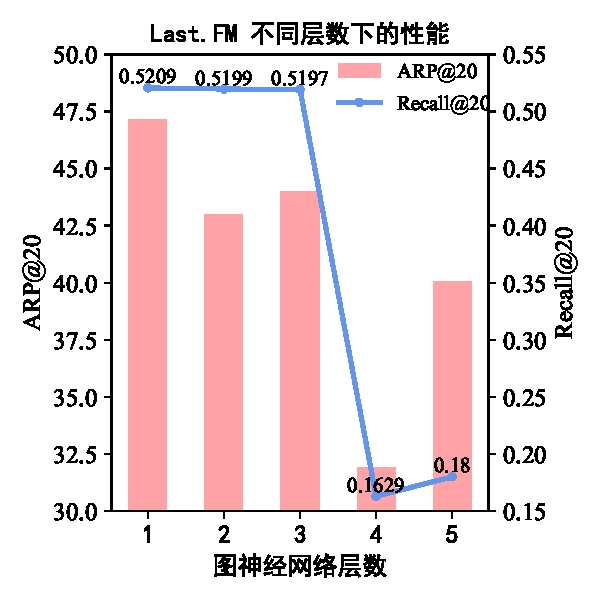
\includegraphics[width=.88\linewidth]{figure/tagcl_param_lastfm_layer.pdf}
      \caption{Last.FM 数据层数对 TAGCL 性能的影响}
      \label{fig:tagcl_param_lastfm_layer}
  \end{subfigure}
  \begin{subfigure}{0.49\linewidth}
    \centering
    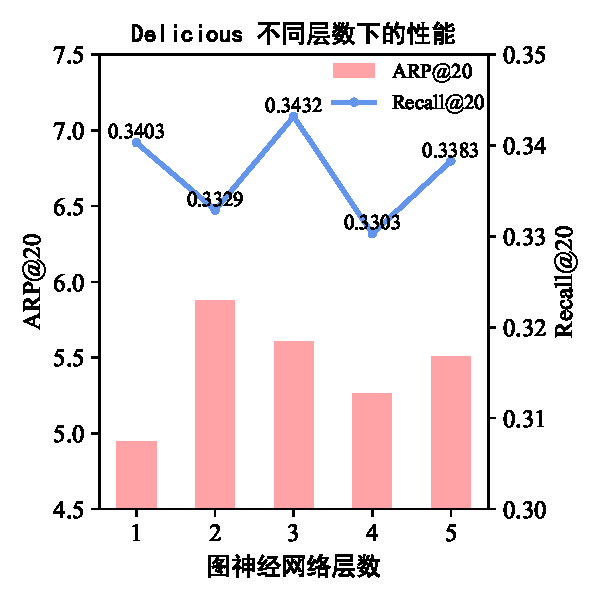
\includegraphics[width=.88\linewidth]{figure/tagcl_param_de_layer.pdf}
    \caption{Delicious 数据层数对 TAGCL 性能的影响}
    \label{fig:tagcl_param_de_layer}
\end{subfigure}
  \caption{图神经网络层数对 TAGCL 性能的影响}
  \label{fig:tagcl_param_layer}
\end{figure}

\begin{figure}[!h]
  \centering
  \begin{subfigure}{0.49\linewidth}
    \centering
    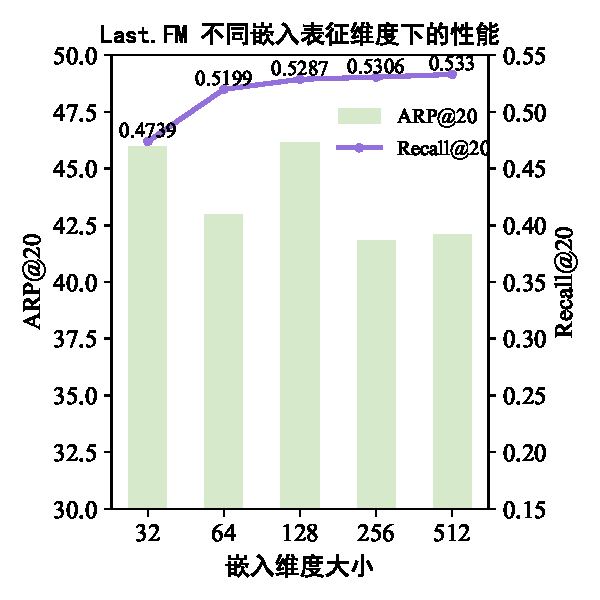
\includegraphics[width=.88\linewidth]{figure/tagcl_param_lastfm_emb.pdf}
    \caption{Last.FM 嵌入表征维度大小对 TAGCL 性能的影响}
    \label{fig:tagcl_param_lastfm_emb}
  \end{subfigure} 
  \begin{subfigure}{0.49\linewidth}
      \centering
      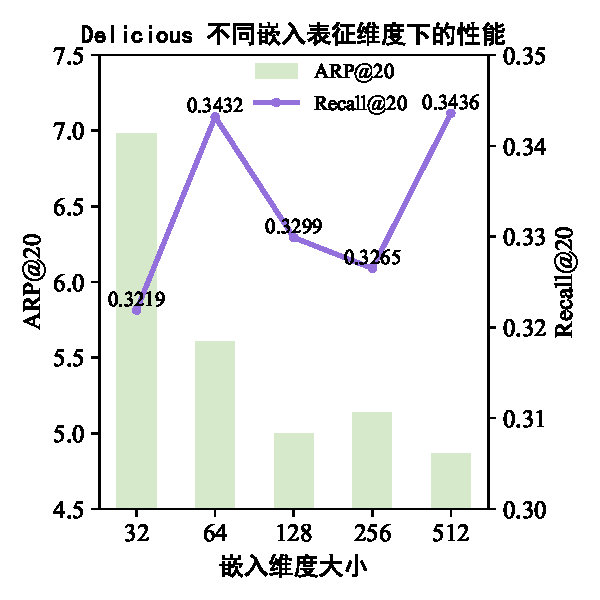
\includegraphics[width=.88\linewidth]{figure/tagcl_param_de_emb.pdf}
      \caption{Delicious 嵌入表征维度大小对 TAGCL 性能的影响}
      \label{fig:tagcl_param_de_emb}
  \end{subfigure}
  \caption{嵌入表征维度大小对 TAGCL 性能的影响}
  \label{fig:tagcl_param_emb}
\end{figure}


此外,我们还研究了嵌入表征的维度大小对 TAGCL 方法的影响。实验结果展示在图~\ref{fig:tagcl_param_emb} 中。在 Last.FM 数据集上(图~\ref{fig:tagcl_param_lastfm_emb}~),我们发现随着嵌入规模的增加,TAGCL 方法的推荐准确率也随之增加。而在 Delicious 数据集上(图~\ref{fig:tagcl_param_de_emb}~),TAGCL 的推荐性能则在嵌入规模变化时表现出较大的波动。特别地,当嵌入规模较大时,TAGCL 方法在 Delicious 数据集上表现更具有公平性。综合考虑性能和效率,我们认为使用 64 的嵌入尺寸是 TAGCL 方法的最佳选择。

\subsubsection{个性化序列长度对模型的影响}
本节旨在探索不同个性化序列长度对 TAGCL 推荐性能的影响。为此,我们分析了数据集 Last.FM 和 Delicious 下,TAGCL 在不同个性化序列长度 $K$ 下与其他基线模型的推荐性能。我们的实验结果显示,TAGCL 在 Recall 和 NDCG 两个指标下,在任意个性化序列长度 $K$ 下均有显著的性能提升,特别是在 NDCG 中,TAGCL 相对于次优模型有约 5\% 的提升。此外,TAGCL 对流行性偏差也有较强的抑制作用,在任意个性化序列长度 $K$ 下均表现出最低的偏差。然而,Delicious 数据集由于数据流行度偏差较小,因此该指标 TAGCL 并没有明显优势。总之,我们的实验结果表明,个性化序列长度 $K$ 对于 TAGCL 推荐性能有着显著的影响,并且该模型能够有效地抑制流行性偏差,提高推荐质量。
\begin{figure}[!h]
  \centering
  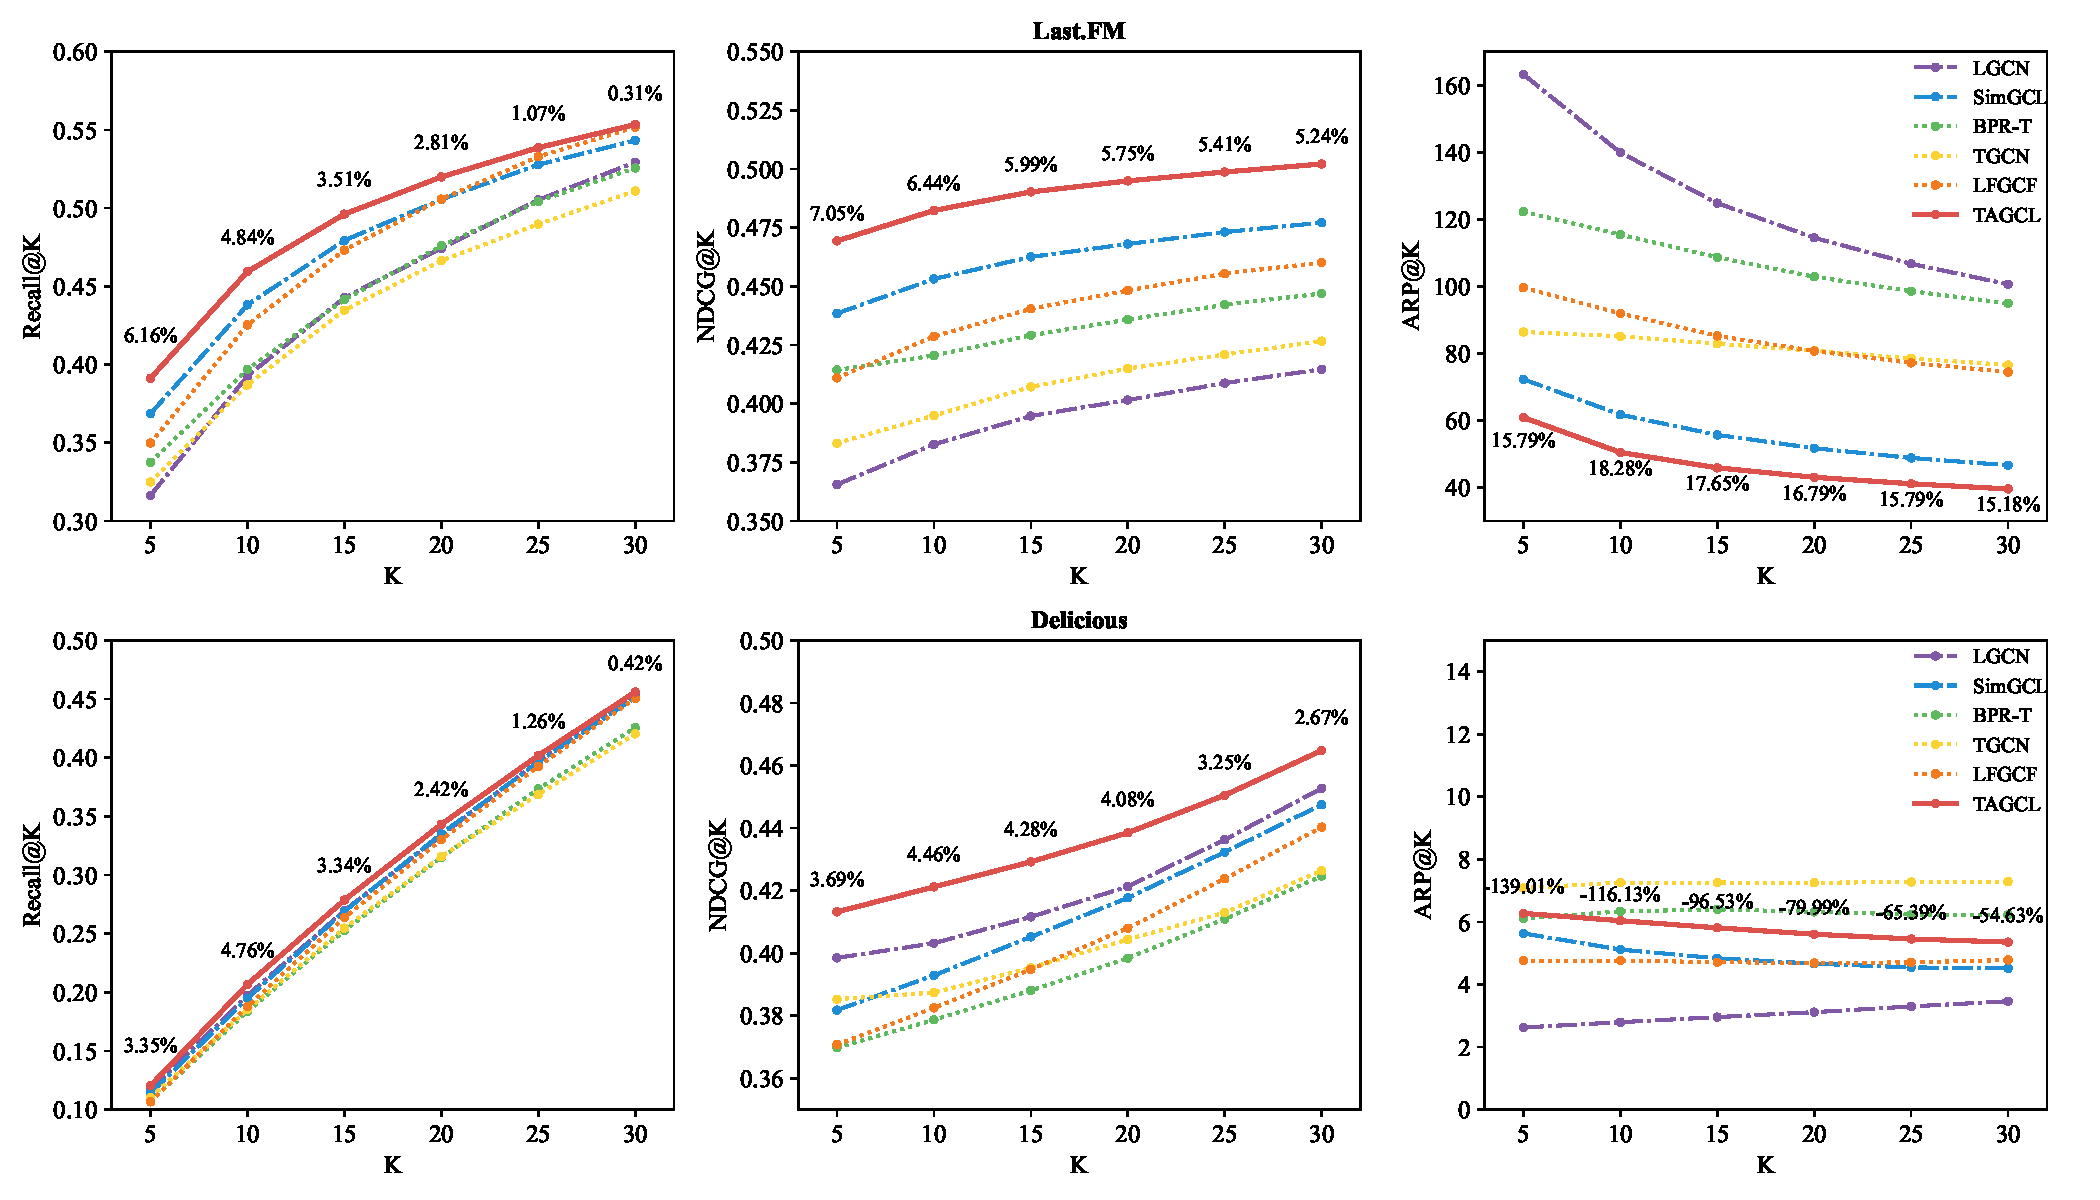
\includegraphics[width=1\linewidth]{figure/topk_comparison.pdf}
  \caption{不同个性化序列长度下的 TAGCL 推荐性能}
  \label{fig:topk}
\end{figure}

\subsection{模型复杂度分析}
本文量化分析了 LFGCF 的参数与推理时间复杂度,并且比较了模型参数量与推理时间。表~\ref{tab:complexity} 展示了 LFGCF 和其他基线模型的参数量与推理时间。与其他标签感知模型相比,LFGCF的参数数量最少,因为它只需要学习用户、项目和标签的嵌入。因此,LFGCF 的参数比一般的模型多。我们的嵌入表征近包含标签嵌入,它提供了大约$0.22 \times 10^6$ 的可训练参数。由于大规模的推荐系列通常对延迟有很高的要求,推理过程中的计算成本很重要。表~\ref{tab:complexity}显示,大多数模型需要大约$0.15s$来推理 Delicious 中的所有测试集。然而,TGCN 明显比其他模型慢,因为它的重特征聚合设计,获得了注意力机制和卷积神经网络。

\begin{table}[!h]
  \centering
    \caption{模型在 Delicious 上的复杂度}
    \label{tab:complexity}
    \begin{tabular}{c|cc|cc}
    \toprule
    \multirow{2}{*}{\textbf{模型}} &
    \multirow{2}{*}{\makecell[c]{参数量 \\ $(\times 10^6$)}} & 
    \multirow{2}{*}{\makecell[c]{相对 \\ 比率 (\%)}} &
    \multirow{2}{*}{\makecell[c]{推理 \\ 时间 (s)}} & 
    \multirow{2}{*}{\makecell[c]{相对 \\ 比率 (\%)}} \\
     & & & 
     \\
      \midrule
       \begin{tabular}[c]{@{}c@{}}
        LightGCN \\ NGCF  \\ LFGCF \\ GNN-PTR \\ TGCN 
        \end{tabular}

        & \begin{tabular}[c]{@{}l@{}}
          \textasciitilde4.33\\  \textasciitilde4.36 \\   \textasciitilde4.55 \\ \textasciitilde4.57 \\ \textasciitilde5.01 
          % 4359168
          % 4334208
          % 5018128
          % 4567104
          % 4558784
        \end{tabular}
        & \begin{tabular}[c]{@{}l@{}}
          -5.18\% \\ -4.58\%   \\ \makecell[c]{-} \\ +0.18\% \\ +9.15\% 
        \end{tabular} 
        & \begin{tabular}[c]{@{}l@{}}
          \textasciitilde0.14 \\ \textasciitilde0.15 \\ \textasciitilde0.13 \\ \textasciitilde0.17 \\ \textasciitilde2.12
        \end{tabular} 
        & \begin{tabular}[c]{@{}l@{}}
          +5.13\% \\ +13.91\% \\ \makecell[c]{-} \\ +16.33\% \\ +93.81\%
        \end{tabular} \\
      \bottomrule
    \end{tabular} 
\end{table}

\subsection{工业数据集上的应用}
为了进一步验证TAGCL的有效性和实用性,我们在社交书签和出版物共享系统BibSonomy的最新版本中进行了离线测试\cite{benz_bibsonomy_2010},其中包含网站的书签数据和出版物的BibTeX数据。我们删除了那些标签分配少于15次的记录,以提高数据质量。BibSonomy-BM 和 BibSonomy-BT 分别指的是整个 BibSonomy 数据集中的书签数据和BibTeX数据。BibSonomy-BM 包含1622320 个交互,涵盖 5996 个用户、8092 个标签和 576232 个项目。BibSonomy-BT 包含 1972556 个交互,涵盖 9721 个用户、11313 个标签和 750514 个项目。它们的稀疏度分别为 99.95\% 和 99.97\%。与我们在之前使用的三个数据集相比,BibSonomy 规模更大,也更为稀疏。我们选择了 LightGCN 作为基线方法,因为它在基线方法中表现优异,并且具有简单性。表~\ref{tab:bibsonomy}~中显示了我们提出的 TAGCL 框架与 LightGCN 的性能比较结果。结果表明,我们提出的 TAGCL 在稀疏的大规模数据集上仍然有效。在 BibSonomy 数据集上,TAGCL 的性能领先优势约为1\%和2\%。与在 Delicious 数据集上的结果相似,TAGCL 提供了准确和高质量的推荐,但推荐的种类和多样性有所减少。我们认为这可能是由于 BibSonomy 和 Delicious 的流行性偏差性较小。

\begin{table}[!h]
  \centering
  \caption{TAGCL 在 BibSonomy 上的应用}
  \label{tab:bibsonomy}
  \begin{tabular}{c|cc|ccc}
    \toprule
    \multirow{2}{*}{\textbf{模型}} &
    \multicolumn{2}{c|}{\textbf{BibSonomy-BM}} &
    \multicolumn{2}{c}{\textbf{BibSonomy-BT}} \\
    \cline{2-5} 
    & \textbf{Rec.@20} & \textbf{ARP.@20} & \textbf{Rec.@20} & \textbf{ARP.@20} \\
    \midrule
    LightGCN & 0.6117 & 1.53 & 0.4810 & 1.39 \\
    TAGCL & 0.6226 & 1.59 & 0.5173 & 1.67 \\
    \bottomrule
  \end{tabular}
\end{table}

\section{本章小结}
本章主要对提出的两个标签感知推荐模型 LFGCF 和 TAGCL 荆襄实验验证和性能对比分析。首先,本章介绍了实验所使用的数据集和数据预处理过程,并将数据集的统计信息与流行度偏差进行可视化。接着阐述具体的实验方法、实验平台和实验流程。在进行多次实验后,整理数据,并对实验结果进行深入分析。实验表明,与现有的通用推荐模型和标签感知推荐模型相比,本文提出的模型在多个评估指标上都有较为显著的性能提升,在三个公开的学术数据集 MovieLens、Last.FM 和 Delicious 上,本文提出的模型 TAGCL 的召回率对比通用推荐模型有 4.6\% 的提升,准确率有 5.0\% 的提升,NDCG有 4.21\% 的提升,MRR 有 1.62\% 的提升。对比标签感知推荐模型,TAGCL 在召回率有 5.18\% 的提升,准确率有 8.0\% 的提升,NDCG有 7.22\% 的提升,MRR 有 5.64\% 的提升。对于数据偏差较大的 MovieLens 与 Last.FM 降低了 17\% 的平均推荐流行度。最后,本文还在一个真实运行的推荐系统数据 BibSonomy 上测试 TAGCL 性能,实验结果证明 TAGCL 对比与基线模型 LightGCN 的召回率领先 1\%。

% 

% \begin{table}
%     \centering
%     \label{tab:movielens_lfgcf_ablation}
%     \caption{数据集 MovieLens 下的 LFGCF 消融实验}
%     \begin{tabular}{ccc}
%         \toprule
%         \textbf{Model} & \textbf{Recall@10} &  \textbf{Recall@20} \\
%         \midrule
%         \begin{tabular}[c]{@{}c@{}}
%             LFGCF-L \\ LFGCF-T \\ LFGCF
%         \end{tabular} 
%         & \begin{tabular}[c]{@{}l@{}}
%             0.217 \\  0.2451\\ 0.25
%         \end{tabular}
%         & \begin{tabular}[c]{@{}l@{}}
%             0.2555  \\ 0.2903 \\  0.2939
%         \end{tabular} \\
%         \bottomrule
%     \end{tabular} 
% \end{table}

% \begin{table}
%     \centering
%     \label{tab:lastfm_lfgcf_ablation}
%     \caption{数据集 Last.FM 下的 LFGCF 消融实验}
%     \begin{tabular}{ccc}
%         \toprule
%         \textbf{Model} & \textbf{Recall@10} &  \textbf{Recall@20} \\
%         \midrule
%         \begin{tabular}[c]{@{}c@{}}
%             LFGCF-L \\ LFGCF-T \\ LFGCF
%         \end{tabular} 
%         & \begin{tabular}[c]{@{}l@{}}
%             0.4208 \\0.4336 \\ 0.4362 
%         \end{tabular}
%         & \begin{tabular}[c]{@{}l@{}}
%             0.4958 \\0.5027 \\ 0.5132
%         \end{tabular} \\
%         \bottomrule
%     \end{tabular} 
% \end{table}


% \begin{table}
%     \centering
%     \label{tab:delicious_lfgcf_ablation}
%     \caption{数据集 Delicious 下的 LFGCF 消融实验}
%     \begin{tabular}{ccc}
%         \toprule
%         \textbf{Model} & \textbf{Recall@10} &  \textbf{Recall@20} \\
%         \midrule
%         \begin{tabular}[c]{@{}c@{}}
%             LFGCF-L \\ LFGCF-T \\ LFGCF
%         \end{tabular} 
%         & \begin{tabular}[c]{@{}l@{}}
%             0.1615 \\ 0.1903 \\ 0.1955
%         \end{tabular}
%         & \begin{tabular}[c]{@{}l@{}}
%             0.2838 \\ 0.3270 \\ 0.3286
%         \end{tabular} \\
%         \bottomrule
%     \end{tabular} 
% \end{table}



% \begin{table}
%     \centering
%     % \label{tab:delicious_lfgcf_ablation}
%     \caption{数据集 MovieLens 下的 TAGCL 消融实验}
%     \begin{tabular}{ccc}
%         \toprule
%         \textbf{Model} & \textbf{Rec.@20} & \textbf{ARP.@20} \\
%         \midrule
%         \begin{tabular}[c]{@{}c@{}}
%             TAGCL-A \\ TAGCL-CL \\ TAGCL-NT \\ TAGCL-T  \\ TAGCL
%           \end{tabular} &
%           \begin{tabular}[c]{@{}c@{}} % recall
%             0.2883 \\ 0.3080 \\ 0.3169 \\ 0.3118 \\ \textbf{0.3180}
%           \end{tabular} & % ARP
%           \begin{tabular}[c]{@{}c@{}}
%             22.89 \\ 20.21 \\ 15.69 \\ 20.11 \\ \textbf{14.96}
%           \end{tabular} \\
%         \bottomrule
%     \end{tabular} 
% \end{table}

% \begin{table}
%     \centering
%     % \label{tab:delicious_lfgcf_ablation}
%     \caption{数据集 Last.FM 下的 TAGCL 消融实验}
%     \begin{tabular}{ccc}
%         \toprule
%         \textbf{Model} & \textbf{Rec.@20} & \textbf{ARP.@20} \\
%         \midrule
%         \begin{tabular}[c]{@{}c@{}}
%             TAGCL-A \\ TAGCL-CL \\ TAGCL-NT \\ TAGCL-T \\ TAGCL
%           \end{tabular} &
%           \begin{tabular}[c]{@{}c@{}} % recall
%             0.4502 \\ 0.4141 \\ \textbf{0.5212} \\ 0.5193 \\ 0.5199
%           \end{tabular} &
%           \begin{tabular}[c]{@{}c@{}} % ARP
%             92.05 \\ 89.42 \\ 43.92 \\ 52.17 \\ \textbf{42.99}
%           \end{tabular} \\
%         \bottomrule
%     \end{tabular} 
% \end{table}

% \begin{table}
%     \centering
%     % \label{tab:delicious_lfgcf_ablation}
%     \caption{数据集 Delicious 下的 TAGCL 消融实验}
%     \begin{tabular}{ccc}
%         \toprule
%         \textbf{Model} & \textbf{Rec.@20} & \textbf{ARP.@20} \\
%         \midrule
%         \begin{tabular}[c]{@{}c@{}}
%             TAGCL-A \\ TAGCL-CL \\ TAGCL-NT \\ TAGCL-T \\ TAGCL
%           \end{tabular} &
%           \begin{tabular}[c]{@{}c@{}} % recall
%             0.3188 \\ 0.3301 \\ 0.3425 \\ 0.3396 \\ \textbf{0.3432}
%           \end{tabular} &
%           \begin{tabular}[c]{@{}c@{}} % ndcg
%             5.33 \\ \textbf{5.24} \\ 5.48 \\ 5.58 \\ 5.61
%           \end{tabular} \\
%         \bottomrule
%     \end{tabular} 
% \end{table}


% \begin{figure*}[!h]
%     \centering
%     \begin{subfigure}{0.49\linewidth}
%         \centering
%         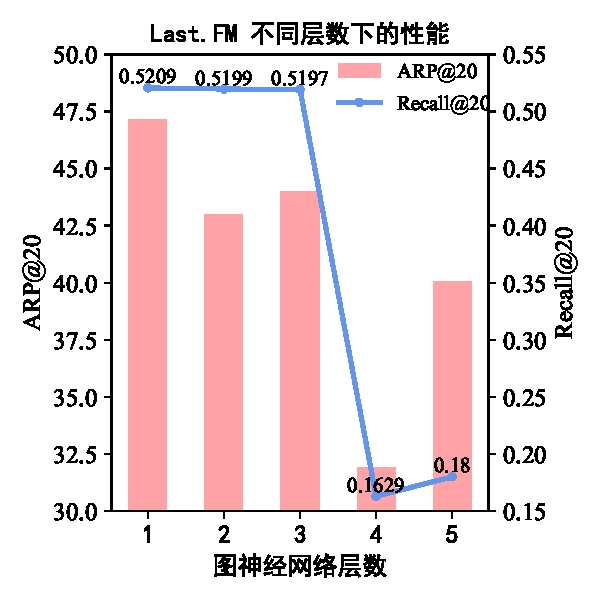
\includegraphics[width=.88\linewidth]{figure/tagcl_param_lastfm_layer.pdf}
%         \caption{layer}
%         \label{fig:tagcl_param_lastfm_layer}
%     \end{subfigure}
%     \begin{subfigure}{0.49\linewidth}
%         \centering
%         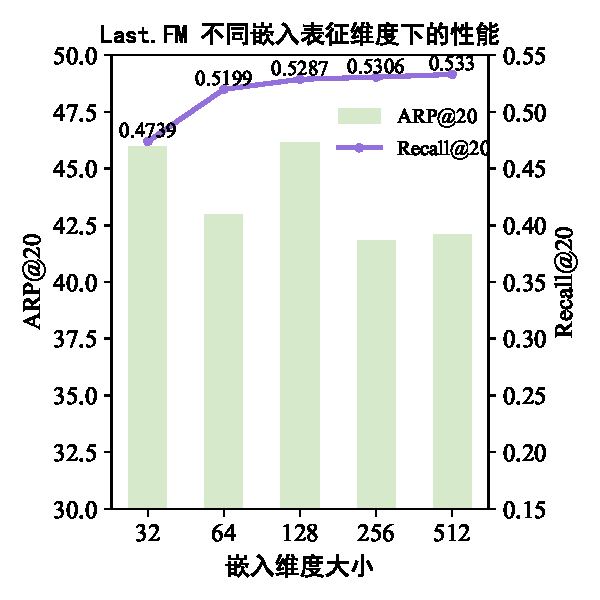
\includegraphics[width=.88\linewidth]{figure/tagcl_param_lastfm_emb.pdf}
%         \caption{emb}
%         \label{fig:tagcl_param_lastfm_emb}
%     \end{subfigure} 
%     \caption{Last.FM 下 TAGCL 的超参数实验}
%     \label{fig:lastfm_tagcl_param}
% \end{figure*}

% \begin{figure*}[!h]
%     \centering
%     \begin{subfigure}{0.49\linewidth}
%         \centering
%         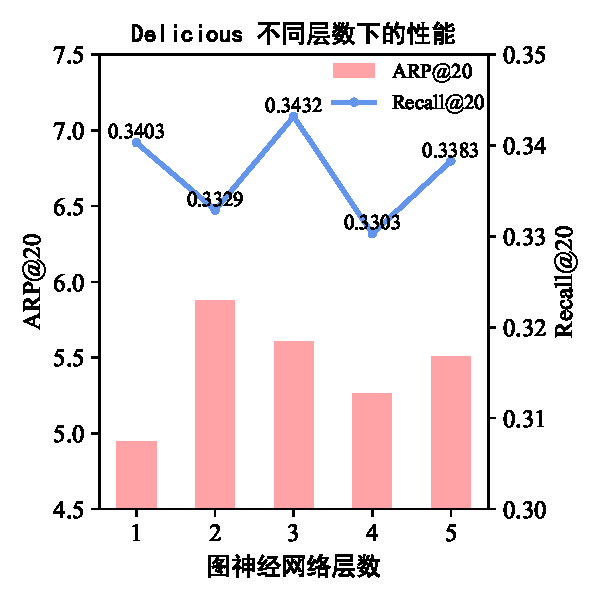
\includegraphics[width=.88\linewidth]{figure/tagcl_param_de_layer.pdf}
%         \caption{layer}
%         \label{fig:tagcl_param_de_layer}
%     \end{subfigure}
%     \begin{subfigure}{0.49\linewidth}
%         \centering
%         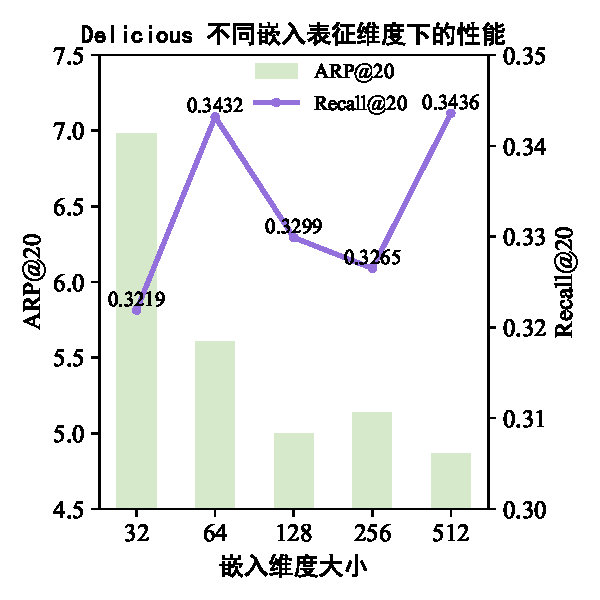
\includegraphics[width=.88\linewidth]{figure/tagcl_param_de_emb.pdf}
%         \caption{emb}
%         \label{fig:tagcl_param_de_emb}
%     \end{subfigure}
%     \caption{Last.FM 下 TAGCL 的超参数实验}
%     \label{fig:de_tagcl_param}
% \end{figure*}

\begin{table}
    \centering
      \caption{模型在 Delicious 上的复杂度}
      \label{tab:complexity}
      \begin{tabular}{c|cc|cc}
      \toprule
      \multirow{2}{*}{\textbf{模型}} &
      \multirow{2}{*}{\makecell[c]{参数量 \\ $(\times 10^6$)}} & 
      \multirow{2}{*}{\makecell[c]{相对 \\ 比率 (\%)}} &
      \multirow{2}{*}{\makecell[c]{推理 \\ 时间 (s)}} & 
      \multirow{2}{*}{\makecell[c]{相对 \\ 比率 (\%)}} \\
       & & & 
       \\
        \midrule
         \begin{tabular}[c]{@{}c@{}}
          LightGCN \\ NGCF  \\ LFGCF \\ GNN-PTR \\ TGCN 
          \end{tabular}
  
          & \begin{tabular}[c]{@{}l@{}}
            \textasciitilde4.33\\  \textasciitilde4.36 \\   \textasciitilde4.55 \\ \textasciitilde4.57 \\ \textasciitilde5.01 
            % 4359168
            % 4334208
            % 5018128
            % 4567104
            % 4558784
          \end{tabular}
          & \begin{tabular}[c]{@{}l@{}}
            -5.18\% \\ -4.58\%   \\ \makecell[c]{-} \\ +0.18\% \\ +9.15\% 
          \end{tabular} 
          & \begin{tabular}[c]{@{}l@{}}
            \textasciitilde0.14 \\ \textasciitilde0.15 \\ \textasciitilde0.13 \\ \textasciitilde0.17 \\ \textasciitilde2.12
          \end{tabular} 
          & \begin{tabular}[c]{@{}l@{}}
            +5.13\% \\ +13.91\% \\ \makecell[c]{-} \\ +16.33\% \\ +93.81\%
          \end{tabular} \\
        \bottomrule
      \end{tabular} 
  \end{table}

  % \begin{table}
  %   \centering
  %   \caption{TAGCL 在 BibSonomy 上的应用}
  %   \label{tab:bibsonomy}
  %   \begin{tabular}{cccccc}
  %     \toprule
  %     \multirow{2}{*}{\textbf{模型}} &
  %     \multicolumn{2}{c}{\textbf{BibSonomy-BM}} &
  %     \multicolumn{2}{c}{\textbf{BibSonomy-BT}} \\
  %     \cline{2-5} 
  %     & \textbf{Rec.@20} & \textbf{ARP.@20} & \textbf{Rec.@20} & \textbf{ARP.@20} \\
  %     \midrule
  %     LightGCN & 0.6117 & 1.53 & 0.4810 & 1.39 \\
  %     TAGCL & 0.6226 & 1.59 & 0.5173 & 1.67 \\
  %     \bottomrule
  %   \end{tabular}
  % \end{table}


  \begin{table}
    \centering
      \caption{模型在 Delicious 上的复杂度}
      \label{tab:complexity}
      \begin{tabular}{c|cc|cc}
      \toprule
      \multirow{2}{*}{\textbf{模型}} &
      \multirow{2}{*}{\makecell[c]{参数量 \\ $(\times 10^6$)}} & 
      \multirow{2}{*}{\makecell[c]{相对 \\ 比率 (\%)}} &
      \multirow{2}{*}{\makecell[c]{推理 \\ 时间 (s)}} & 
      \multirow{2}{*}{\makecell[c]{相对 \\ 比率 (\%)}} \\
       & & & 
       \\
        \midrule
         \begin{tabular}[c]{@{}c@{}}
          LightGCN \\ NGCF  \\ LFGCF \\ GNN-PTR \\ TGCN 
          \end{tabular}
  
          & \begin{tabular}[c]{@{}l@{}}
            \textasciitilde4.33\\  \textasciitilde4.36 \\   \textasciitilde4.55 \\ \textasciitilde4.57 \\ \textasciitilde5.01 
            % 4359168
            % 4334208
            % 5018128
            % 4567104
            % 4558784
          \end{tabular}
          & \begin{tabular}[c]{@{}l@{}}
            -5.18\% \\ -4.58\%   \\ \makecell[c]{-} \\ +0.18\% \\ +9.15\% 
          \end{tabular} 
          & \begin{tabular}[c]{@{}l@{}}
            \textasciitilde0.14 \\ \textasciitilde0.15 \\ \textasciitilde0.13 \\ \textasciitilde0.17 \\ \textasciitilde2.12
          \end{tabular} 
          & \begin{tabular}[c]{@{}l@{}}
            +5.13\% \\ +13.91\% \\ \makecell[c]{-} \\ +16.33\% \\ +93.81\%
          \end{tabular} \\
        \bottomrule
      \end{tabular} 
  \end{table}


  


\chapter[结论与展望]{结论与展望}
\label{chap:conclusion}

\newpage
\pagestyle{fancy}
% \begin{center}
% \heiti\sanhao {参考文献}
% \end{center}

\addcontentsline{toc}{chapter}{参考文献}
% \printbibliography[title={参考文献}]
\bibliography{mybibfile}
% \printbibliography[heading=bibliography,title=参考文献]

\newpage
\pagestyle{fancy}
\begin{center}
\heiti\sanhao {硕士研究生期间的科研成果}
\end{center}

\addcontentsline{toc}{chapter}{硕士研究生期间的科研成果}

论文:

\textbf{XU C}, ZHANG Y, WANG W, DONG L. Pursuit and evasion strategy of a differential game based on deep reinforcement learning[J]. Frontiers in Bioengineering and Biotechnology, 2022, 10: 827408.

ZHANG Y, \textbf{XU C}, WU X, ZHANG Y, DONG L, WANG W. LFGCF: Light folksonomy graph collaborative filtering for tag-aware recommendation[J]. Expert Systems with Applications, 2022, Under Review.

\textbf{XU C}, ZHANG Y, CHEN H, DONG L, WANG W. A fairness-aware graph contrastive learning recommender framework for social tagging systems[J]. Information Sciences, 2023: 119064.

Chen H, \textbf{XU C}, ZHENG L, WANG W. Diffusion-based graph generative methods[J]. ACM Computing Surveys, 2023, Under Review.

\textbf{XU C}, WANG W, CHEN H. Geometric-facilitated Denoising Diffusion Model for 3D Molecule Generation[C]//Proceedings of the AAAI Conference on Artificial Intelligence, 2024, Under Review.

\

课题:

面向分布式异构计算系统内存池化关键技术,国家重点研发计划之先进计算与新兴软件。

% 混合模型及改进EM算法的理论与应用. 浙江省自然科学基金 Y19A010012. 排名: 3/5.

\

竞赛:

“华为杯”第十八届中国研究生数学建模竞赛,三等奖,排名: 1/3。

第五届全国应用统计专业学位研究生案例大赛,三等奖,排名: 1/3。

OGB-LSC @NeurIPS 2022 (PCQM4Mv2 Track),NO.11,排名:1/5。

第十一届“泰迪杯”数据挖掘挑战赛,三等奖,排名:1/3。

\end{document}